\section{Sistema propuesto.}

En esta sección vamos a exponer los requisitos extraidos del análisis de la descripción del proyecto, que se van a 
especificar en los requisitos funcionales y no funcionales, los caso de uso, sus actores y diagramas de clase y secuencia.
Se comentará sobre la planificación y presupuesto que se ha llevado a cabo.

\subsection{Análisis de requerimientos.}

\subsubsection{Requisitos funcionales.}

\paragraph{RF-1. Gestión de usuarios.} Habrá dos actores principales: los usuarios finales y el administrador.

\begin{itemize}
    \item[] RF-1.1. El usuario podrá solicitar darse de alta.
    \item[] RF-1.2. El usuario podrá solicitar darse de baja.
    \item[] RF-1.3. El administrador podrá dar de alta a un usuario en la red Blockchain.
    \item[] RF-1.4. El administrador podrá revocar el certificado de un usuario en la red Blockchain.
    \item[] RF-1.5. El administrador podrá renovar el certificado de un usuario en la red Blockchain.
\end{itemize}

\paragraph{RF-2. Gestión de dispositivos.} El sistema permitirá la gestión de dispositivos IoT de los usuarios, dentro de 
la aplicación. Podemos catalogar los dispositivos entre: sensores y actuadores.

\begin{itemize}
    \item[] RF-2.1. El usuario tendrá permitido añadir un dispositivo indicando un nombre, su número serial y su dirección
    IP.
    \item[] RF-2.2. El usuario podrá establecer un valor númerico al sensor como valor de entrada y se comprobará las 
    condiciones de sus enlaces en el cual se encuentre involucrado.
    \item[] RF-2.3. El usuario no podrá establecer un valor númerico al actuador, se dejará por defecto el -1.
    \item[] RF-2.4. El usuario podrá borrar el dispositivo de la red, indicando el número serial.
    \item[] RF-2.5. El usuario podrá consultar todos los dispositivos añadidos a la aplicación.
    \item[] RF-2.6. El usuario podrá consultar los datos del dispositivo indicando el número serial.
    \item[] RF-2.7. El usuario podrá consultar el historial de un dispositivos indicando el número serial.
\end{itemize}

\paragraph{RF-3. Gestión de enlaces.} El sistema permitirá la gestión de enlaces de dispositivos IoT dentro de la 
aplicación. Los enlaces  viene a representar la relación que hay entre un sensor y un actuador, mediante una condición de 
activación.

\begin{itemize}
    \item[] RF-3.1. El usuario tendrá permitido añadir un enlace indicando los dispositivos que lo forman (el número 
    serial del sensor y el número serial del actuador), la región donde se encuentre los dispositivo, y una condición, 
    formada por una variable, acompañado de un operador de comparación y un valor númerico. Al añadirse, tendrá su estado 
    activado por defecto.
    \item[] RF-3.2. El usuario podrá actualizar un enlace, indicando su ID (hash del número serial del sensor y el 
    actuador). Podrá cambiar la condición y la región.
    \item[] RF-3.3. El usuario podrá borrar un enlace, indicando su ID.
    \item[] RF-3.4. El usuario podrá habilitar un enlace, y se mandará una señal de activación al actuador. 
    \item[] RF-3.5. El usuario podrá deshabilitar un enlace, y se mandará una señal de desactivación al actuador.
    \item[] RF-3.6. El usuario podrá consultar todos los enlaces añadidos a la aplicación.
    \item[] RF-3.7. El usuario podrá consultar los datos del enlace indicando el ID del mismo.
    \item[] RF-3.8. El usuario podrá consultar el historial de un enlace indicando el ID del mismo.
\end{itemize}

\subsubsection{Requisitos no funcionales.}

\begin{itemize}
    \item[] RNF-1. La aplicación ha de ser accesible desde fuera de la red local, con cualquier dispositivo, smartphone, 
    table, portatil o sobremesa
    \item[] RNF-2. La aplicación tiene que ser compatible con diferentes navegadores.
    \item[] RNF-3. Se establecerán conexiones seguras dentro de la aplicación, cifrando las peticiones HTTP.
    \item[] RNF-4. La aplicación tiene que cumplir los criterios de PWA, tiene que trabajar de forma offline, mandar
    notificaciones y soportar la sincronización en segundo plano.
    \item[] RNF-5. La aplicación tiene que adaptarse a cualquier dimension de pantalla, es decir, tiene que ser 
    responsive.
    \item[] RNF-6. La aplicación tiene que cumplir niveles de rendimiento, accesibilidad y SEO\footnote{ SEO significa 
    Search Engine Optimization (optimización de motores de búsqueda), que es la práctica de aumentar la cantidad y la 
    calidad del tráfico se un sitio web a través de los resultados orgánicos de los motores de búsqueda 
    \cite{what-is-seo}. 
    \label{fnlabel}} aceptables, utilizando la aplicación LightHouse\footnote{ Es una herramienta elaborada por Google de 
    código abierto para mejorar la calidad de las páginas web \cite{lighthouse}. \label{fnlabel}}.
    \item[] RNF-7. La interfaz ha de ser clara e intuitiva.
    \item[] RNF-8. Se realizarán test a la aplicación.
    \item[] RNF-9. No se requerirá de conocimientos previos para el uso de la aplicación.
    \item[] RNF-10. La API tiene que ser accesible desde la aplicación, para realizar cualquier petición directamente
    a la red Blockchain.
\end{itemize}

\subsection{Especificación.}

\subsubsection{Actores de los casos de uso.}

\begin{itemize}
    \item \textbf{Entorno}: es el actor vinculado al medio ambiente, se incluye lo referente al aire, la temperatura, la 
    humedad, el tiempo atmosférico, etc. Los sensores se van a encargar de recoger eso datos del exterior y manejarlos.
    \item \textbf{Dispositivo}: es el actor que realiza un mecanismo con una función específica. Podemos diferenciar entre 
    sensores y actuadores. Nos refirimos a los dispositivos de IoT.
    \item \textbf{Enlace}: es el actor que está formado por dos dispositivos, un sensor y un actuador. Un enlace va a estar 
    condicionado por el cumplimiento de la condición establecida por el usuario. Por defecto, el enlace creado va a estar 
    habilitado. Cuando un sensor recibe un valor, se comprobará cada uno de sus enlaces establecidos. En el caso de que se 
    cumpla la condición, el enlace se habilita y se mandará una señal de activación al actuador.
    \item \textbf{Usuario}: es el actor que puede usar las principales funcionalidades que ofrece la aplicación una vez que 
    tenga un certificado de autoridad dentro de la red Blockchain. Podrá llevar una gestión de sus dispositivos y enlaces 
    dentro de la aplicación y gracias a la tecnología Blockchain, podrá ver toda la trazabilidad de las transacciones 
    realizadas y resistente a modificaciones.
    \item \textbf{Administrador}: es el actor encargado de la gestión de usuarios, se encargará de administrar todo lo 
    relacionado con los certificados de autoridad de cada usuario del sistema.
\end{itemize}

\subsubsection{Diagramas de casos de uso.}

\begin{itemize}
    \item Gestión de usuarios.
    
    \vspace{5mm}

    \begin{figure}[h!]
        \centering
        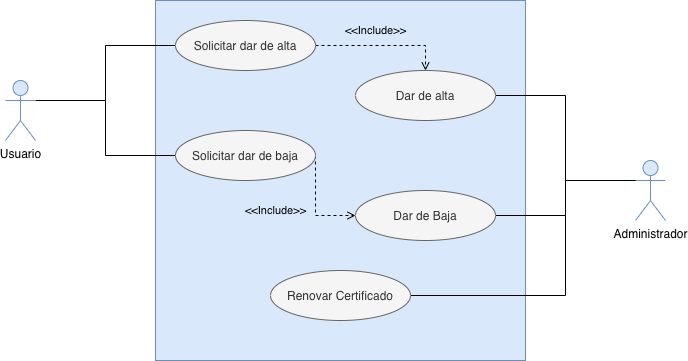
\includegraphics[width=12cm]{imagenes/diagramas/diagrama_gestion_usuarios}
        \caption{Diagrama de casos de uso de Gestión de usuarios.}
        \label{fig:gestion-de-usuarios}
    \end{figure}

    \newpage

    \item Gestión de dispositivos.
    
    \vspace{5mm}

    \begin{figure}[h!]
        \centering
        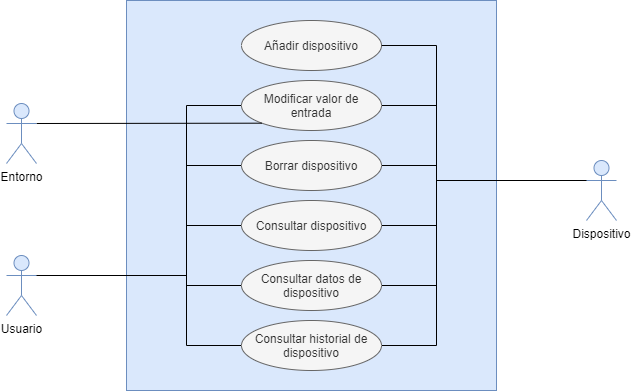
\includegraphics[width=12cm]{imagenes/diagramas/diagrama_gestion_dispositivos}
        \caption{Diagrama de casos de uso de Gestión de dispositivos.}
        \label{fig:gestion-de-dispositivos}
    \end{figure}

    \item Gestión de enlaces.
    
    \vspace{5mm}

    \begin{figure}[b!]
        \centering
        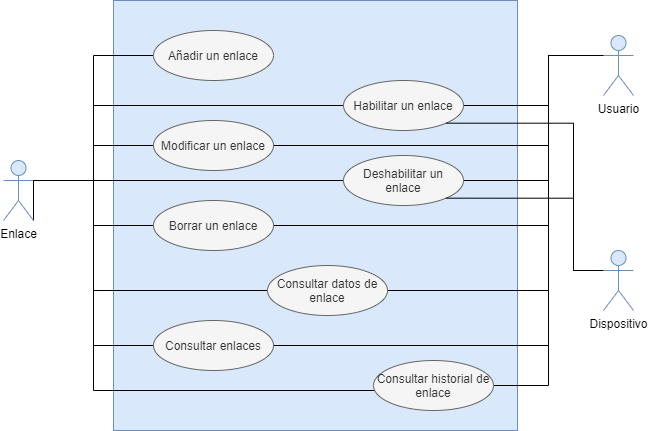
\includegraphics[width=12cm]{imagenes/diagramas/diagrama_gestion_enlaces}
        \caption{Diagrama de casos de uso de Gestión de enlaces.}
        \label{fig:gestion-de-enlaces}
    \end{figure}
\end{itemize}

\newpage

\subsubsection{Especificación de casos de uso.}

\begin{itemize}
    \item Caso de uso 1: Solicitar dar de alta a un usuario.
    
    \begin{table}[h!]
        \centering
        \begin{tabular}{|l|p{0.753\textwidth}|}
            \hline
            \textbf{Casos de Uso}   &   Solicitar dar de alta a un usuario (CU\_01). \\
            \hline 
            \textbf{Actores}        &   Usuario (Principal) y Administrador (Secundario). \\ 
            \hline 
            \textbf{Tipo}           &   Primario y esencial. \\
            \hline
            \textbf{Referencias}    &   RF-1.1., RF-1.3. \\ 
            \hline
            \textbf{Precondición}   &   El usuario no debe de tener un certificado de autoridad asociada en la red. \\ 
            \hline
            \textbf{Postcondición}  &   El usuario tendrá un certificado de autoridad. \\ 
            \hline
        \end{tabular}
        
        \vspace{5mm}
        
        \begin{tabular}{|p{\textwidth}|}
            \hline
            \rowcolor{SeaGreen} \textbf{Propósito} \\
            \hline
            \multicolumn{1}{|p{12cm}|}{El usuario obtendrá el certificado de autoridad para poder realizar operaciones en 
            el sistema, firmando las transacciones.} \\ [0.5ex]
            \hline
        \end{tabular}
        
        \vspace{5mm}
        
        \begin{tabular}{|p{\textwidth}|}
            \hline
            \rowcolor{SeaGreen} \textbf{Resumen} \\
            \hline
            \multicolumn{1}{|p{12cm}|}{El usuario solicitará al administrador la petición de darse de alta del sistem. El 
            administrador se encargará de crear el certificado de autoridad del usuario y lo guardará en la cartera, para 
            que el usuario pueda realizar acciones en la aplicación.} \\ [0.5ex]
            \hline
        \end{tabular}
        
        \vspace{5mm}
        
        \begin{tabular}{|p{0.01\textwidth}|p{0.438\textwidth}|p{0.01\textwidth}|p{0.438\textwidth}|}
            \cline{1-4}
            \rowcolor{SeaGreen} \multicolumn{4}{|l|}{\textbf{Curso Normal}} \\
            \cline{1-4}
            \textbf{1} & Usuario: manda petición de darse de alta. & & \\
            \hline
            \textbf{2} & Administrador: manda petición para crear el certificado de autoridad. & & \\
            \hline
             & & \textbf{3} & El sistema crea el certificado de autoridad. \\
            \hline
             & & \textbf{4} & El sistema guarda el certificado en la cartera (wallet). \\
            \hline
        \end{tabular}
        
        \vspace{5mm}
        
        \begin{tabular}{|p{0.224\textwidth}|p{0.224\textwidth}|p{0.224\textwidth}|p{0.224\textwidth}|}
            \cline{1-4}
            \rowcolor{SeaGreen} \multicolumn{4}{|l|}{\textbf{Otros datos}} \\
            \cline{1-4}
            \textbf{Frecuencia \newline esperada} & Media & \textbf{Rendimiento} &  \\
            \hline
            \textbf{Importancia} & Alta & \textbf{Urgencia} & Alta \\
            \hline
            \textbf{Estado} & & \textbf{Estabilidad} & Alta \\
            \hline
        \end{tabular}
        
        \caption{Caso de uso 1: Solicitar dar de alta a un usuario.}
        \label{table:caso-de-uso-1}
    \end{table}
    
    \newpage
    
    \item Caso de uso 2: Solicitar dar de baja a un usuario. 
    
    \begin{table}[h!]
        \centering
        \begin{tabular}{|l|p{0.753\textwidth}|}
            \hline
            \textbf{Casos de Uso}   &   Solicitar dar de baja a un usuario (CU\_02). \\
            \hline 
            \textbf{Actores}        &   Usuario (Principal) y Administrador (Secundario). \\ 
            \hline 
            \textbf{Tipo}           &   Primario y esencial. \\
            \hline
            \textbf{Referencias}    &   RF-1.2., RF-1.4.\\ 
            \hline
            \textbf{Precondición}   &   El usuario debe de tener un certificado de autoridad asociada en la red.\\ 
            \hline
            \textbf{Postcondición}  &   El usuario no tendra un certificado de autoridad.\\ 
            \hline
        \end{tabular}
        
        \vspace{5mm}
        
        \begin{tabular}{|p{\textwidth}|}
            \hline
            \rowcolor{SeaGreen} \textbf{Propósito} \\
            \hline
            \multicolumn{1}{|p{12cm}|}{El usuario perderá el certificado de autoridad y por tanto no podrá realizar
            ninguna operación en la red.} \\ [0.5ex]
            \hline
        \end{tabular}
        
        \vspace{5mm}
        
        \begin{tabular}{|p{\textwidth}|}
            \hline
            \rowcolor{SeaGreen} \textbf{Resumen} \\
            \hline
            \multicolumn{1}{|p{12cm}|}{El usuario solicitará al administrador la petición de darse de baja del sistema. El 
            administrador se encargará de revocar el certificado de autoridad del usuario. El certificado de autoridad se 
            borrará de la cartera (wallet).} \\ [0.5ex]
            \hline
        \end{tabular}
        
        \vspace{5mm}
        
        \begin{tabular}{|p{0.01\textwidth}|p{0.438\textwidth}|p{0.01\textwidth}|p{0.438\textwidth}|}
            \cline{1-4}
            \rowcolor{SeaGreen} \multicolumn{4}{|l|}{\textbf{Curso Normal}} \\
            \cline{1-4}
            \textbf{1} & Usuario: manda petición de darse de baja. & & \\
            \hline
            \textbf{2} & Administrador: manda petición para revocar el certificado de autoridad. & & \\
            \hline
             & & \textbf{3} & El sistema revoca el certificado de autoridad. \\
            \hline
             & & \textbf{4} & El sistema borra el certificado de la cartera (wallet). \\
            \hline
        \end{tabular}
        
        \vspace{5mm}
        
        \begin{tabular}{|p{0.224\textwidth}|p{0.224\textwidth}|p{0.224\textwidth}|p{0.224\textwidth}|}
            \cline{1-4}
            \rowcolor{SeaGreen} \multicolumn{4}{|l|}{\textbf{Otros datos}} \\
            \cline{1-4}
            \textbf{Frecuencia \newline esperada} & Media & \textbf{Rendimiento} &  \\
            \hline
            \textbf{Importancia} & Alta & \textbf{Urgencia} & Alta \\
            \hline
            \textbf{Estado} & & \textbf{Estabilidad} & Alta \\
            \hline
        \end{tabular}
        
        \caption{Caso de uso 2: Solicitar dar de baja a un usuario.}
        \label{table:caso-de-uso-2}
    \end{table}

    \newpage

    \item Caso de uso 3: Dar de alta a un usuario. 
    
    \begin{table}[h!]
        \centering
        \begin{tabular}{|l|p{0.753\textwidth}|}
            \hline
            \textbf{Casos de Uso}   &   Dar de alta a un usuario (CU\_03). \\
            \hline 
            \textbf{Actores}        &   Administrador (Principal) y Usuario (Secundario)\\ 
            \hline 
            \textbf{Tipo}           &   Primario y esencial. \\ 
            \hline
            \textbf{Referencias}    &   RF-1.3., RF-1.1. \\ 
            \hline
            \textbf{Precondición}   &   El Administrador debe de recibir una solicitud de dar de alta. \\ 
            \hline
            \textbf{Postcondición}  &   El certificado de autoridad se guarda en el sistema. \\ 
            \hline
        \end{tabular}
        
        \vspace{5mm}
        
        \begin{tabular}{|p{\textwidth}|}
            \hline
            \rowcolor{SeaGreen} \textbf{Propósito} \\
            \hline
            \multicolumn{1}{|p{12cm}|}{El administrador mandará la solicitud al sistema, para crear el certificado de 
            autoridad.} \\ [0.5ex]
            \hline
        \end{tabular}
        
        \vspace{5mm}
        
        \begin{tabular}{|p{\textwidth}|}
            \hline
            \rowcolor{SeaGreen} \textbf{Resumen} \\
            \hline
            \multicolumn{1}{|p{12cm}|}{El administrador se encargará de crear el certificado de autoridad del usuario y
            lo guardará en la cartera, para que el usuario pueda realizar acciones en la aplicación.} \\ [0.5ex]
            \hline
        \end{tabular}
        
        \vspace{5mm}
        
        \begin{tabular}{|p{0.01\textwidth}|p{0.438\textwidth}|p{0.01\textwidth}|p{0.438\textwidth}|}
            \cline{1-4}
            \rowcolor{SeaGreen} \multicolumn{4}{|l|}{\textbf{Curso Normal}} \\
            \cline{1-4}
            \textbf{1} & Administrador: manda petición para crear el certificado de autoridad. &  &  \\
            \hline
             & & \textbf{2} & El sistema crea el certificado de autoridad. \\
            \hline
             & & \textbf{3} & El sistema guarda el certificado en la cartera (wallet). \\
            \hline
        \end{tabular}
        
        \vspace{5mm}
        
        \begin{tabular}{|p{0.224\textwidth}|p{0.224\textwidth}|p{0.224\textwidth}|p{0.224\textwidth}|}
            \cline{1-4}
            \rowcolor{SeaGreen} \multicolumn{4}{|l|}{\textbf{Otros datos}} \\
            \cline{1-4}
            \textbf{Frecuencia \newline esperada} & Media & \textbf{Rendimiento} &  \\
            \hline
            \textbf{Importancia} & Alta & \textbf{Urgencia} & Alta \\
            \hline
            \textbf{Estado} & & \textbf{Estabilidad} & Alta \\
            \hline
        \end{tabular}
        
        \caption{Caso de uso 3: Dar de alta a un usuario.}
        \label{table:caso-de-uso-3}
    \end{table}
    
    \newpage
    
    \item Caso de uso 4: Dar de baja a un usuario.
    
    \begin{table}[h!]
        \centering
        \begin{tabular}{|l|p{0.753\textwidth}|}
            \hline
            \textbf{Casos de Uso}   &   Dar de baja a un usuario (CU\_04). \\
            \hline 
            \textbf{Actores}        &   Administrador (Principal) y Usuario (Secundario). \\ 
            \hline 
            \textbf{Tipo}           &   Primario y esencial. \\ 
            \hline
            \textbf{Referencias}    &   RF-1.4., RF-1.2.\\ 
            \hline
            \textbf{Precondición}   &   Debe de existir un certificado de autoridad asociado al usuario.\\ 
            \hline
            \textbf{Postcondición}  &   Se revoca el certificado.\\ 
            \hline
        \end{tabular}
        
        \vspace{5mm}
        
        \begin{tabular}{|p{\textwidth}|}
            \hline
            \rowcolor{SeaGreen} \textbf{Propósito} \\
            \hline
            \multicolumn{1}{|p{12cm}|}{El administrador mandará la solicitud al sistema, para revocar el certificado
            de autoridad del usuario.} \\ [0.5ex]
            \hline
        \end{tabular}
        
        \vspace{5mm}
        
        \begin{tabular}{|p{\textwidth}|}
            \hline
            \rowcolor{SeaGreen} \textbf{Resumen} \\
            \hline
            \multicolumn{1}{|p{12cm}|}{El administrador se encargará de revocar el certificado de autoridad del usuario.
            El certificado de autoridad se borrará de la cartera (wallet).} \\ [0.5ex]
            \hline
        \end{tabular}
        
        \vspace{5mm}
        
        \begin{tabular}{|p{0.01\textwidth}|p{0.438\textwidth}|p{0.01\textwidth}|p{0.438\textwidth}|}
            \cline{1-4}
            \rowcolor{SeaGreen} \multicolumn{4}{|l|}{\textbf{Curso Normal}} \\
            \cline{1-4}
            \textbf{1} & Administrador: manda petición para revocar el certificado de autoridad. &  &  \\
            \hline
             & & \textbf{2} & El sistema revoca el certificado de autoridad. \\
            \hline
             & & \textbf{3} & El sistema borra el certificado de autoridad de la carter (wallet). \\
            \hline
        \end{tabular}
        
        \vspace{5mm}
        
        \begin{tabular}{|p{0.224\textwidth}|p{0.224\textwidth}|p{0.224\textwidth}|p{0.224\textwidth}|}
            \cline{1-4}
            \rowcolor{SeaGreen} \multicolumn{4}{|l|}{\textbf{Otros datos}} \\
            \cline{1-4}
            \textbf{Frecuencia \newline esperada} & Media & \textbf{Rendimiento} &  \\
            \hline
            \textbf{Importancia} & Alta & \textbf{Urgencia} & Alta \\
            \hline
            \textbf{Estado} & & \textbf{Estabilidad} & Alta \\
            \hline
        \end{tabular}
        
        \caption{Caso de uso 4: Dar de baja a un usuario.}
        \label{table:caso-de-uso-4}
    \end{table}
    
    \newpage

    \item Caso de uso 5: Renovar el certificado de autoridad del usuario.
    
    \begin{table}[h!]
        \centering
        \begin{tabular}{|l|p{0.753\textwidth}|}
            \hline
            \textbf{Casos de Uso}   &   Renovar el certificado de autoridad del usuario (CU\_05). \\
            \hline 
            \textbf{Actores}        &   Administrador (Principal) y Usuario (Secundario). \\ 
            \hline 
            \textbf{Tipo}           &   Primario y esencial. \\ 
            \hline
            \textbf{Referencias}    &   RF-1.5., RF-1.4.\\ 
            \hline
            \textbf{Precondición}   &  Debe de existir un certificado de autoridad asociado al usuario y tiene que 
            haber expirado la fecha de finalización del certificado. \\ 
            \hline
            \textbf{Postcondición}  &  Se emite un nuevo certificado de autoridad para el usuario. \\ 
            \hline
        \end{tabular}
        
        \vspace{5mm}
        
        \begin{tabular}{|p{\textwidth}|}
            \hline
            \rowcolor{SeaGreen} \textbf{Propósito} \\
            \hline
            \multicolumn{1}{|p{12cm}|}{El administrador mandará la solicitud al sistema, para renovar el 
            certificado de autoridad del usuario.} \\ [0.5ex]
            \hline
        \end{tabular}
        
        \vspace{5mm}
        
        \begin{tabular}{|p{\textwidth}|}
            \hline
            \rowcolor{SeaGreen} \textbf{Resumen} \\
            \hline
            \multicolumn{1}{|p{12cm}|}{El administrado manda la petición de renovación, que consiste en la emisión de un 
            nuevo certificado para que el sistema (CA) extienda la vida útil de la misma más allá de la fecha de 
            finalización del certificado original.} \\ [0.5ex]
            \hline
        \end{tabular}
        
        \vspace{5mm}
        
        \begin{tabular}{|p{0.01\textwidth}|p{0.438\textwidth}|p{0.01\textwidth}|p{0.438\textwidth}|}
            \cline{1-4}
            \rowcolor{SeaGreen} \multicolumn{4}{|l|}{\textbf{Curso Normal}} \\
            \cline{1-4}
            \textbf{1} & Administrador: comprueba la fecha de expiración del certificado. &  &  \\
            \hline
            \textbf{2} & Administrador: manda la petición para renovar el certificado. & & \\
            \hline
             & & \textbf{3} & El sistema renueva el certificado de autoridad. \\
            \hline
             & & \textbf{4} & El sistema guarda el certificado en la cartera (wallet). \\
             \hline
        \end{tabular}
        
        \vspace{5mm}
        
        \begin{tabular}{|p{0.224\textwidth}|p{0.224\textwidth}|p{0.224\textwidth}|p{0.224\textwidth}|}
            \cline{1-4}
            \rowcolor{SeaGreen} \multicolumn{4}{|l|}{\textbf{Otros datos}} \\
            \cline{1-4}
            \textbf{Frecuencia \newline esperada} & Media & \textbf{Rendimiento} & Alta \\
            \hline
            \textbf{Importancia} & Alta & \textbf{Urgencia} & Media \\
            \hline
            \textbf{Estado} & & \textbf{Estabilidad} & Alta \\
            \hline
        \end{tabular}
        
        \caption{Caso de uso 5: Renovar el certificado de autoridad del usuario.}
        \label{table:caso-de-uso-5}
    \end{table}
    
    \newpage
    
    \item Caso de uso 6: Añadir un dispositivo.
    
    \begin{table}[h!]
        \centering
        \begin{tabular}{|l|p{0.753\textwidth}|}
            \hline
            \textbf{Casos de Uso}   &   Añadir un dispositivo (CU\_06). \\
            \hline 
            \textbf{Actores}        &   Dispositivo (Principal). \\ 
            \hline 
            \textbf{Tipo}           &   Primario y esencial. \\ 
            \hline
            \textbf{Referencias}    &   RF-2.1. \\ 
            \hline
            \textbf{Precondición}   &   No debe de existir un dispositivo con el mismo número serial o direccón IP en el 
            sistema. \\ 
            \hline
            \textbf{Postcondición}  &   Se añade el nuevo dispositivo con valor -1. \\ 
            \hline
        \end{tabular}
        
        \vspace{5mm}
        
        \begin{tabular}{|p{\textwidth}|}
            \hline
            \rowcolor{SeaGreen} \textbf{Propósito} \\
            \hline
            \multicolumn{1}{|p{12cm}|}{El usuario podrá añadir un dispositivo que no esté registrado anteriormente.} \\ [0.5ex]
            \hline
        \end{tabular}
        
        \vspace{5mm}
        
        \begin{tabular}{|p{\textwidth}|}
            \hline
            \rowcolor{SeaGreen} \textbf{Resumen} \\
            \hline
            \multicolumn{1}{|p{12cm}|}{El usuario introducirá los datos asociados con el dispositivo, que son el nombre, 
            el número serial y la dirección IP. Se comprobará que no haya un dispositivo existente con el número serial y 
            la dirección IP iguales, en ese caso se añadirá el dispositivo con el atributo valor -1 por defecto.} \\ [0.5ex]
            \hline
        \end{tabular}
        
        \vspace{5mm}
        
        \begin{tabular}{|p{0.01\textwidth}|p{0.438\textwidth}|p{0.01\textwidth}|p{0.438\textwidth}|}
            \cline{1-4}
            \rowcolor{SeaGreen} \multicolumn{4}{|l|}{\textbf{Curso Normal}} \\
            \cline{1-4}
            \textbf{1} & Usuario: introducirá los datos del dispositivo. &  &  \\
            \hline
             & & \textbf{2} & El sistema comprueba los datos introducidos. \\
            \hline
             & & \textbf{3} & El sistema valida los datos y guarda el nuevo dispositivo en la red Blockchain. \\
            \hline
        \end{tabular}
        
        \vspace{5mm}
        
        \begin{tabular}{|p{0.224\textwidth}|p{0.224\textwidth}|p{0.224\textwidth}|p{0.224\textwidth}|}
            \cline{1-4}
            \rowcolor{SeaGreen} \multicolumn{4}{|l|}{\textbf{Otros datos}} \\
            \cline{1-4}
            \textbf{Frecuencia \newline esperada} & Alta & \textbf{Rendimiento} & Media \\
            \hline
            \textbf{Importancia} & Media & \textbf{Urgencia} & Baja \\
            \hline
            \textbf{Estado} & & \textbf{Estabilidad} & Alta \\
            \hline
        \end{tabular}
        
        \caption{Caso de uso 6: Añadir un dispositivo.}
        \label{table:caso-de-uso-6}
    \end{table}
    
    \newpage

    \item Caso de uso 7: Modificar el valor de entrada de un sensor.
    
    \begin{table}[h!]
        \centering
        \begin{tabular}{|l|p{0.753\textwidth}|}
            \hline
            \textbf{Casos de Uso}   &   Modificar el valor de entrada de un sensor (CU\_07). \\
            \hline 
            \textbf{Actores}        &   Dispositivo (Principal), Entorno (Secundario) y Usuario (Secundario). \\ 
            \hline 
            \textbf{Tipo}           &   Primario y esencial. \\ 
            \hline
            \textbf{Referencias}    &   RF-2.2., RF-2.3. \\ 
            \hline
            \textbf{Precondición}   &   El dispositivo debe de estar registrado en el sistema y tiene que ser un sensor. \\ 
            \hline
            \textbf{Postcondición}  &   El valor del sensor se habrá modificado y se habrá comprobado las condiciones de 
            sus enlaces. \\ 
            \hline
        \end{tabular}
        
        \vspace{5mm}
        
        \begin{tabular}{|p{\textwidth}|}
            \hline
            \rowcolor{SeaGreen} \textbf{Propósito} \\
            \hline
            \multicolumn{1}{|p{12cm}|}{El entorno o el usuario podrá modificar los valores de entrada de un sensor para 
            habilitar o deshabilitar enlaces en el cual se encuentre involucrado.} \\ [0.5ex]
            \hline
        \end{tabular}
        
        \vspace{5mm}
        
        \begin{tabular}{|p{\textwidth}|}
            \hline
            \rowcolor{SeaGreen} \textbf{Resumen} \\
            \hline
            \multicolumn{1}{|p{12cm}|}{Los datos que se obtiene del entorno o los datos que introduce un usuario a un 
            sensor, el sensor guardará el dato obtenido y se comprobará los enlaces que esté involucrado el dispositivo, 
            para habilitar o deshabilitar el enlace de acuerdo a la condición establecida en el enlace.} \\ [0.5ex]
            \hline
        \end{tabular}
        
        \vspace{5mm}
        
        \begin{tabular}{|p{0.01\textwidth}|p{0.438\textwidth}|p{0.01\textwidth}|p{0.438\textwidth}|}
            \cline{1-4}
            \rowcolor{SeaGreen} \multicolumn{4}{|l|}{\textbf{Curso Normal}} \\
            \cline{1-4}
            \textbf{1} & Entorno o Usuario: Introduce el dato de entrada al sensor. &  &  \\
            \hline
            \textbf{2} & Dispositivo (Sensor): guarda el valor de entrada. &  & \\
            \hline
             & & \textbf{3} & El sistema guarda el dato. \\
            \hline
             & & \textbf{4} & El sistema comprueba los enlaces. \\
            \hline
        \end{tabular}
        
        \vspace{5mm}
        
        \begin{tabular}{|p{0.224\textwidth}|p{0.224\textwidth}|p{0.224\textwidth}|p{0.224\textwidth}|}
            \cline{1-4}
            \rowcolor{SeaGreen} \multicolumn{4}{|l|}{\textbf{Otros datos}} \\
            \cline{1-4}
            \textbf{Frecuencia \newline esperada} & Muy Alta & \textbf{Rendimiento} & Alta \\
            \hline
            \textbf{Importancia} & Muy Alta & \textbf{Urgencia} & Alta\\
            \hline
            \textbf{Estado} & & \textbf{Estabilidad} & Alta \\
            \hline
        \end{tabular}
        
        \caption{Caso de uso 7: Modificar el valor de entrada de un sensor.}
        \label{table:caso-de-uso-7}
    \end{table}
    
    \newpage
    
    \item Caso de uso 8: Borrar un dispositivo.
    
    \begin{table}[h!]
        \centering
        \begin{tabular}{|l|p{0.753\textwidth}|}
            \hline
            \textbf{Casos de Uso}   &   Borrar un dispositivo (CU\_08). \\
            \hline 
            \textbf{Actores}        &   Dispositivo (Principal) y Usuario (Secundario). \\ 
            \hline 
            \textbf{Tipo}           &   Primario y esencial. \\ 
            \hline
            \textbf{Referencias}    &   RF-2.4.\\ 
            \hline
            \textbf{Precondición}   &   El dispositivo de estar registrado en el sistema. \\ 
            \hline
            \textbf{Postcondición}  &   Se ha borrado el dispositivo. \\ 
            \hline
        \end{tabular}
        
        \vspace{5mm}
        
        \begin{tabular}{|p{\textwidth}|}
            \hline
            \rowcolor{SeaGreen} \textbf{Propósito} \\
            \hline
            \multicolumn{1}{|p{12cm}|}{El usuario podrá borrar el dispositivo seleccionado. } \\ [0.5ex]
            \hline
        \end{tabular}
        
        \vspace{5mm}
        
        \begin{tabular}{|p{\textwidth}|}
            \hline
            \rowcolor{SeaGreen} \textbf{Resumen} \\
            \hline
            \multicolumn{1}{|p{12cm}|}{El sistema facilitará al usuario la opción de borrar un dispositivo.} \\ [0.5ex]
            \hline
        \end{tabular}
        
        \vspace{5mm}
        
        \begin{tabular}{|p{0.01\textwidth}|p{0.438\textwidth}|p{0.01\textwidth}|p{0.438\textwidth}|}
            \cline{1-4}
            \rowcolor{SeaGreen} \multicolumn{4}{|l|}{\textbf{Curso Normal}} \\
            \cline{1-4}
            \textbf{1} & Usuario: Selecciona el dispositivo a borrar. &  &  \\
            \hline
             & & \textbf{2} & El sistema borra el dispositivo. \\
            \hline
        \end{tabular}
        
        \vspace{5mm}
        
        \begin{tabular}{|p{0.224\textwidth}|p{0.224\textwidth}|p{0.224\textwidth}|p{0.224\textwidth}|}
            \cline{1-4}
            \rowcolor{SeaGreen} \multicolumn{4}{|l|}{\textbf{Otros datos}} \\
            \cline{1-4}
            \textbf{Frecuencia \newline esperada} & Baja & \textbf{Rendimiento} & Media \\
            \hline
            \textbf{Importancia} & Media & \textbf{Urgencia} & Baja \\
            \hline
            \textbf{Estado} & & \textbf{Estabilidad} & Alta \\
            \hline
        \end{tabular}
        
        \caption{Caso de uso 8: Borrar un dispositivo.}
        \label{table:caso-de-uso-8}
    \end{table}
    
    \newpage

    \item Caso de uso 9: Consultar dispositivos.
    
    \begin{table}[h!]
        \centering
        \begin{tabular}{|l|p{0.753\textwidth}|}
            \hline
            \textbf{Casos de Uso}   &   Consultar dispositivos (CU\_09). \\
            \hline 
            \textbf{Actores}        &   Dispositivo (Principal) y Usuario (Secundario). \\ 
            \hline 
            \textbf{Tipo}           &   Primario y esencial. \\ 
            \hline
            \textbf{Referencias}    &   RF-2.5. \\ 
            \hline
            \textbf{Precondición}   &   \\ 
            \hline
            \textbf{Postcondición}  &   El usuario obtendrá una lista de dispositivos. \\ 
            \hline
        \end{tabular}
        
        \vspace{5mm}
        
        \begin{tabular}{|p{\textwidth}|}
            \hline
            \rowcolor{SeaGreen} \textbf{Propósito} \\
            \hline
            \multicolumn{1}{|p{12cm}|}{Permitir al usuario poder consultar los dispositivos guardados.} \\ [0.5ex]
            \hline
        \end{tabular}
        
        \vspace{5mm}
        
        \begin{tabular}{|p{\textwidth}|}
            \hline
            \rowcolor{SeaGreen} \textbf{Resumen} \\
            \hline
            \multicolumn{1}{|p{12cm}|}{El usuario podrá consultar los dispositivos guardados y ver los datos de cada uno 
            de ellos.} \\ [0.5ex]
            \hline
        \end{tabular}
        
        \vspace{5mm}
        
        \begin{tabular}{|p{0.01\textwidth}|p{0.438\textwidth}|p{0.01\textwidth}|p{0.438\textwidth}|}
            \cline{1-4}
            \rowcolor{SeaGreen} \multicolumn{4}{|l|}{\textbf{Curso Normal}} \\
            \cline{1-4}
            \textbf{1} & Usuario: solicita consultar los dispositivos. &  &  \\
            \hline
             & & \textbf{2} & El sistema devuelve una lista de los dispositivos guardados. \\
            \hline
        \end{tabular}
        
        \vspace{5mm}
        
        \begin{tabular}{|p{0.224\textwidth}|p{0.224\textwidth}|p{0.224\textwidth}|p{0.224\textwidth}|}
            \cline{1-4}
            \rowcolor{SeaGreen} \multicolumn{4}{|l|}{\textbf{Otros datos}} \\
            \cline{1-4}
            \textbf{Frecuencia \newline esperada} & Alta & \textbf{Rendimiento} & Media \\
            \hline
            \textbf{Importancia} & Media & \textbf{Urgencia} & Baja \\
            \hline
            \textbf{Estado} & & \textbf{Estabilidad} & Alta \\
            \hline
        \end{tabular}
        
        \caption{Caso de uso 9: Consultar dispositivos.}
        \label{table:caso-de-uso-9}
    \end{table}
    
    \newpage
    
    \item Caso de uso 10: Consultar los datos de un dispositivo.
    
    \begin{table}[h!]
        \centering
        \begin{tabular}{|l|p{0.753\textwidth}|}
            \hline
            \textbf{Casos de Uso}   &   Consultar los datos de un dispositivo (CU\_10). \\
            \hline 
            \textbf{Actores}        &   Dispositivo (Principal) y Usuario (Secundario). \\ 
            \hline 
            \textbf{Tipo}           &   Primario y esencial. \\ 
            \hline
            \textbf{Referencias}    &   RF-2.6. \\ 
            \hline
            \textbf{Precondición}   &   El dispositivo debe de estar registrado en el sistema. \\ 
            \hline
            \textbf{Postcondición}  &   El usuario obtendrá los datos del dispositivo. \\ 
            \hline
        \end{tabular}
        
        \vspace{5mm}
        
        \begin{tabular}{|p{\textwidth}|}
            \hline
            \rowcolor{SeaGreen} \textbf{Propósito} \\
            \hline
            \multicolumn{1}{|p{12cm}|}{Permitir al usuario poder consultar los datos de un dispositivo.} \\ [0.5ex]
            \hline
        \end{tabular}
        
        \vspace{5mm}
        
        \begin{tabular}{|p{\textwidth}|}
            \hline
            \rowcolor{SeaGreen} \textbf{Resumen} \\
            \hline
            \multicolumn{1}{|p{12cm}|}{El usuario seleccionará el dispositivo que quiere consultar y el sistema se lo 
            proporcionará.} \\ [0.5ex]
            \hline
        \end{tabular}
        
        \vspace{5mm}
        
        \begin{tabular}{|p{0.01\textwidth}|p{0.438\textwidth}|p{0.01\textwidth}|p{0.438\textwidth}|}
            \cline{1-4}
            \rowcolor{SeaGreen} \multicolumn{4}{|l|}{\textbf{Curso Normal}} \\
            \cline{1-4}
            \textbf{1} & Usuario: solicita consultar los datos del dispositivo. &  &  \\
            \hline
             & & \textbf{2} & El sistema comprueba si existe el dispositivo. \\
            \hline
             & & \textbf{3} & El sistema devuelve los datos del dispositivo guardado. \\
            \hline
        \end{tabular}
        
        \vspace{5mm}
        
        \begin{tabular}{|p{0.224\textwidth}|p{0.224\textwidth}|p{0.224\textwidth}|p{0.224\textwidth}|}
            \cline{1-4}
            \rowcolor{SeaGreen} \multicolumn{4}{|l|}{\textbf{Otros datos}} \\
            \cline{1-4}
            \textbf{Frecuencia \newline esperada} & Alta & \textbf{Rendimiento} & Media \\
            \hline
            \textbf{Importancia} & Media & \textbf{Urgencia} & Baja\\
            \hline
            \textbf{Estado} & & \textbf{Estabilidad} & Alta \\
            \hline
        \end{tabular}
        
        \caption{Caso de uso 10: Consultar los datos de un dispositivo.}
        \label{table:caso-de-uso-10}
    \end{table}
    
    \newpage

    \item Caso de uso 11: Consultar el historial de un dispositivo.
    
    \begin{table}[h!]
        \centering
        \begin{tabular}{|l|p{0.753\textwidth}|}
            \hline
            \textbf{Casos de Uso}   &   Consultar el historial de un dispositivo (CU\_11). \\
            \hline 
            \textbf{Actores}        &   Dispositivo (Principal) y Usuario (Secundario). \\ 
            \hline 
            \textbf{Tipo}           &   Primario y esencial. \\
            \hline
            \textbf{Referencias}    &   RF-2.7. \\ 
            \hline
            \textbf{Precondición}   &   El dispositivo debe de estar registrado en el sistema. \\ 
            \hline
            \textbf{Postcondición}  &   El usuario obtendrá el historial de un dispositivo. \\ 
            \hline
        \end{tabular}
        
        \vspace{5mm}
        
        \begin{tabular}{|p{\textwidth}|}
            \hline
            \rowcolor{SeaGreen} \textbf{Propósito} \\
            \hline
            \multicolumn{1}{|p{12cm}|}{Permitir al usuario consultar el historial de un dispositivo.} \\ [0.5ex]
            \hline
        \end{tabular}
        
        \vspace{5mm}
        
        \begin{tabular}{|p{\textwidth}|}
            \hline
            \rowcolor{SeaGreen} \textbf{Resumen} \\
            \hline
            \multicolumn{1}{|p{12cm}|}{Gracias al tecnología Blockchain, se puede obtener todas las transacciones
            realizadas y con ello poder ver los diferentes cambios que ha tenido un dispositivo, desde su momento
            de creación hasta ahora.} \\ [0.5ex]
            \hline
        \end{tabular}
        
        \vspace{5mm}
        
        \begin{tabular}{|p{0.01\textwidth}|p{0.438\textwidth}|p{0.01\textwidth}|p{0.438\textwidth}|}
            \cline{1-4}
            \rowcolor{SeaGreen} \multicolumn{4}{|l|}{\textbf{Curso Normal}} \\
            \cline{1-4}
            \textbf{1} & Usuario: solicita consultar el historial del dispositivo. &  &  \\
            \hline
             & & \textbf{2} & El sistema comprueba si existe el dispositivo. \\
            \hline
             & & \textbf{3} & El sistema devuelve el historial del dispositivo guardado. \\
            \hline
        \end{tabular}
        
        \vspace{5mm}
        
        \begin{tabular}{|p{0.224\textwidth}|p{0.224\textwidth}|p{0.224\textwidth}|p{0.224\textwidth}|}
            \cline{1-4}
            \rowcolor{SeaGreen} \multicolumn{4}{|l|}{\textbf{Otros datos}} \\
            \cline{1-4}
            \textbf{Frecuencia \newline esperada} & Alta & \textbf{Rendimiento} & Media \\
            \hline
            \textbf{Importancia} & Media & \textbf{Urgencia} & Baja \\
            \hline
            \textbf{Estado} & & \textbf{Estabilidad} & Alta \\
            \hline
        \end{tabular}
        
        \caption{Caso de uso 11: Consultar el historial de un dispositivo.}
        \label{table:caso-de-uso-11}
    \end{table}
    
    \newpage
    
    \item Caso de uso 12: Añadir un enlace.
    
    \begin{table}[h!]
        \centering
        \begin{tabular}{|l|p{0.753\textwidth}|}
            \hline
            \textbf{Casos de Uso}   &   Añadir un enlace (CU\_12). \\
            \hline 
            \textbf{Actores}        &   Enlace (Principal). \\ 
            \hline 
            \textbf{Tipo}           &   Primario y esencial. \\ 
            \hline
            \textbf{Referencias}    &   RF-3.1. \\ 
            \hline
            \textbf{Precondición}   &   No debe de existir un enlace con el mismo sensor y actuador, además deben
            de existir ambos dispositivos. \\ 
            \hline
            \textbf{Postcondición}  &   Se añade el nuevo enlace y está habilitado. \\ 
            \hline
        \end{tabular}
        
        \vspace{5mm}
        
        \begin{tabular}{|p{\textwidth}|}
            \hline
            \rowcolor{SeaGreen} \textbf{Propósito} \\
            \hline
            \multicolumn{1}{|p{12cm}|}{El usuario podrá añadir un nuevo enlace que no esté regitrado anteriormente.} \\ [0.5ex]
            \hline
        \end{tabular}
        
        \vspace{5mm}
        
        \begin{tabular}{|p{\textwidth}|}
            \hline
            \rowcolor{SeaGreen} \textbf{Resumen} \\
            \hline
            \multicolumn{1}{|p{12cm}|}{El usuario introducirá el número serial del sensor y del actuador, una región 
            dónde se localice dicho enlace y por último, una condición. Dicha condición va a estar formado por una 
            variable "value", acompañado de un operador de comparación y un valor numérico. Se generará un ID que es 
            el hash del número serial del sensor y el actuador.} \\ [0.5ex]
            \hline
        \end{tabular}
        
        \vspace{5mm}
        
        \begin{tabular}{|p{0.01\textwidth}|p{0.438\textwidth}|p{0.01\textwidth}|p{0.438\textwidth}|}
            \cline{1-4}
            \rowcolor{SeaGreen} \multicolumn{4}{|l|}{\textbf{Curso Normal}} \\
            \cline{1-4}
            \textbf{1} & Usuario: introducirá los datos del enlace. &  &  \\
            \hline
            & & \textbf{2} & El sistema comprueba los datos introducidos. \\
            \hline
            & & \textbf{3} & El sistema valida los datos y guarda el nuevo enlace en la red Blockchain. \\
            \hline
        \end{tabular}
        
        \vspace{5mm}
        
        \begin{tabular}{|p{0.224\textwidth}|p{0.224\textwidth}|p{0.224\textwidth}|p{0.224\textwidth}|}
            \cline{1-4}
            \rowcolor{SeaGreen} \multicolumn{4}{|l|}{\textbf{Otros datos}} \\
            \cline{1-4}
            \textbf{Frecuencia \newline esperada} & Alta & \textbf{Rendimiento} & Media \\
            \hline
            \textbf{Importancia} & Media & \textbf{Urgencia} & Baja \\
            \hline
            \textbf{Estado} & & \textbf{Estabilidad} & Alta \\
            \hline
        \end{tabular}
        
        \caption{Caso de uso 12: Añadir un enlace.}
        \label{table:caso-de-uso-12}
    \end{table}
    
    \newpage

    \item Caso de uso 13: Modificar un enlace.
    
    \begin{table}[h!]
        \centering
        \begin{tabular}{|l|p{0.753\textwidth}|}
            \hline
            \textbf{Casos de Uso}   &   Modificar un enlace (CU\_13). \\
            \hline 
            \textbf{Actores}        &   Enlace (Principal) y Usuario (Secundario). \\ 
            \hline 
            \textbf{Tipo}           &   Primario y esencial. \\
            \hline
            \textbf{Referencias}    &   RF-3.2., RF-3.4., RF-3.5. \\ 
            \hline
            \textbf{Precondición}   &   El enlace debe de estar registrado en el sistema. \\ 
            \hline
            \textbf{Postcondición}  &   Los datos del enlace se habrán actualizado. \\ 
            \hline
        \end{tabular}
        
        \vspace{5mm}
        
        \begin{tabular}{|p{\textwidth}|}
            \hline
            \rowcolor{SeaGreen} \textbf{Propósito} \\
            \hline
            \multicolumn{1}{|p{12cm}|}{El usuario podrá modificar la región, el estado o la condición del enlace.} \\ [0.5ex]
            \hline
        \end{tabular}
        
        \vspace{5mm}
        
        \begin{tabular}{|p{\textwidth}|}
            \hline
            \rowcolor{SeaGreen} \textbf{Resumen} \\
            \hline
            \multicolumn{1}{|p{12cm}|}{El usuario, verá los datos del enlace, modificará lo que desee y el sistema 
            actualizará esos datos.} \\ [0.5ex]
            \hline
        \end{tabular}
        
        \vspace{5mm}
        
        \begin{tabular}{|p{0.01\textwidth}|p{0.438\textwidth}|p{0.01\textwidth}|p{0.438\textwidth}|}
            \cline{1-4}
            \rowcolor{SeaGreen} \multicolumn{4}{|l|}{\textbf{Curso Normal}} \\
            \cline{1-4}
            \textbf{1} & Usuario: introducirá los datos del enlace. &  &  \\
            \hline
            & & \textbf{2} & El sistema comprueba los datos introducidos. \\
            \hline
            & & \textbf{3} & El sistema valida los datos y guarda el nuevo enlace en la red Blockchain. \\
            \hline
        \end{tabular}
        
        \vspace{5mm}
        
        \begin{tabular}{|p{0.224\textwidth}|p{0.224\textwidth}|p{0.224\textwidth}|p{0.224\textwidth}|}
            \cline{1-4}
            \rowcolor{SeaGreen} \multicolumn{4}{|l|}{\textbf{Otros datos}} \\
            \cline{1-4}
            \textbf{Frecuencia \newline esperada} & Muy Alta & \textbf{Rendimiento} & Alta \\
            \hline
            \textbf{Importancia} & Muy Alta & \textbf{Urgencia} & Alta\\
            \hline
            \textbf{Estado} & & \textbf{Estabilidad} & Alta \\
            \hline
        \end{tabular}
        
        \caption{Caso de uso 13: Modificar un enlace.}
        \label{table:caso-de-uso-13}
    \end{table}
    
    \newpage

    \item Caso de uso 14: Borrar un enlace.
    
    \begin{table}[h!]
        \centering
        \begin{tabular}{|l|p{0.753\textwidth}|}
            \hline
            \textbf{Casos de Uso}   &   Borrar un enlace (CU\_14). \\
            \hline 
            \textbf{Actores}        &   Enlace (Principal) y Usuario (Secundario). \\ 
            \hline 
            \textbf{Tipo}           &   Primario y esencial. \\ 
            \hline
            \textbf{Referencias}    &   RF-3.3. \\ 
            \hline
            \textbf{Precondición}   &   El enlace de estar registrado en el sistema. \\ 
            \hline
            \textbf{Postcondición}  &   Se ha borrado el enlace. \\ 
            \hline
        \end{tabular}
        
        \vspace{5mm}
        
        \begin{tabular}{|p{\textwidth}|}
            \hline
            \rowcolor{SeaGreen} \textbf{Propósito} \\
            \hline
            \multicolumn{1}{|p{12cm}|}{El usuario podrá borrar el enlace seleccionado. } \\ [0.5ex]
            \hline
        \end{tabular}
        
        \vspace{5mm}
        
        \begin{tabular}{|p{\textwidth}|}
            \hline
            \rowcolor{SeaGreen} \textbf{Resumen} \\
            \hline
            \multicolumn{1}{|p{12cm}|}{El sistema facilitará al usuario la opción de borrar un enlace.} \\ [0.5ex]
            \hline
        \end{tabular}
        
        \vspace{5mm}
        
        \begin{tabular}{|p{0.01\textwidth}|p{0.438\textwidth}|p{0.01\textwidth}|p{0.438\textwidth}|}
            \cline{1-4}
            \rowcolor{SeaGreen} \multicolumn{4}{|l|}{\textbf{Curso Normal}} \\
            \cline{1-4}
            \textbf{1} & Usuario: Selecciona el enlace a borrar. &  &  \\
            \hline
             & & \textbf{2} & El sistema borra el enlace. \\
            \hline
        \end{tabular}
        
        \vspace{5mm}
        
        \begin{tabular}{|p{0.224\textwidth}|p{0.224\textwidth}|p{0.224\textwidth}|p{0.224\textwidth}|}
            \cline{1-4}
            \rowcolor{SeaGreen} \multicolumn{4}{|l|}{\textbf{Otros datos}} \\
            \cline{1-4}
            \textbf{Frecuencia \newline esperada} & Baja & \textbf{Rendimiento} & Media \\
            \hline
            \textbf{Importancia} & Media & \textbf{Urgencia} & Baja \\
            \hline
            \textbf{Estado} & & \textbf{Estabilidad} & Alta \\
            \hline
        \end{tabular}
        
        \caption{Caso de uso 14: Borrar un enlace.}
        \label{table:caso-de-uso-14}
    \end{table}
    
    \newpage
    
    \item Caso de uso 15: Habilitar un enlace.
    
    \begin{table}[h!]
        \centering
        \begin{tabular}{|l|p{0.753\textwidth}|}
            \hline
            \textbf{Casos de Uso}   &   Habilitar un enlace (CU\_15). \\
            \hline 
            \textbf{Actores}        &   Enlace (Principal), Dispositivo (Secundario) y Usuario (Secundario). \\ 
            \hline 
            \textbf{Tipo}           &   Primario y esencial. \\ 
            \hline
            \textbf{Referencias}    &   RF-3.4. \\ 
            \hline
            \textbf{Precondición}   &   El enlace debe de estar registrado en el sistema. \\ 
            \hline
            \textbf{Postcondición}  &   El enlace se habilita. \\ 
            \hline
        \end{tabular}
        
        \vspace{5mm}
        
        \begin{tabular}{|p{\textwidth}|}
            \hline
            \rowcolor{SeaGreen} \textbf{Propósito} \\
            \hline
            \multicolumn{1}{|p{12cm}|}{El usuario y el sensor, podrán habilitar el enlace.} \\ [0.5ex]
            \hline
        \end{tabular}
        
        \vspace{5mm}
        
        \begin{tabular}{|p{\textwidth}|}
            \hline
            \rowcolor{SeaGreen} \textbf{Resumen} \\
            \hline
            \multicolumn{1}{|p{12cm}|}{El enlace se podrá habilitar dependiendo de el valor de entrada recibido por el
            sensor, en el caso de que se cumpla la condición. También el usuario podrá habilitar el enlace. Cuando se 
            habilite, se mandará una petición HTTP para activar el actuador.} \\ [0.5ex]
            \hline
        \end{tabular}
        
        \vspace{5mm}
        
        \begin{tabular}{|p{0.01\textwidth}|p{0.438\textwidth}|p{0.01\textwidth}|p{0.438\textwidth}|}
            \cline{1-4}
            \rowcolor{SeaGreen} \multicolumn{4}{|l|}{\textbf{Curso Normal}} \\
            \cline{1-4}
            \textbf{1} & Dispositivo o Usuario: solicita habilitar el enlace. &  &  \\
            \hline
             & & \textbf{2} & El sistema habilita el enlace. \\
            \hline
             & & \textbf{3} & El sistema manda la petición HTTP. \\
            \hline
        \end{tabular}
        
        \vspace{5mm}
        
        \begin{tabular}{|p{0.224\textwidth}|p{0.224\textwidth}|p{0.224\textwidth}|p{0.224\textwidth}|}
            \cline{1-4}
            \rowcolor{SeaGreen} \multicolumn{4}{|l|}{\textbf{Otros datos}} \\
            \cline{1-4}
            \textbf{Frecuencia \newline esperada} & Muy Alta & \textbf{Rendimiento} & Alta \\
            \hline
            \textbf{Importancia} & Muy Alta & \textbf{Urgencia} & Alta\\
            \hline
            \textbf{Estado} & & \textbf{Estabilidad} & Alta \\
            \hline
        \end{tabular}
        
        \caption{Caso de uso 15: Habilitar un enlace.}
        \label{table:caso-de-uso-15}
    \end{table}
    
    \newpage

    \item Caso de uso 16: Deshabilitar un enlace.
    
    \begin{table}[h!]
        \centering
        \begin{tabular}{|l|p{0.753\textwidth}|}
            \hline
            \textbf{Casos de Uso}   &   Deshabilitar un enlace (CU\_16). \\
            \hline 
            \textbf{Actores}        &   Enlace (Principal), Dispositivo (Secundario) y Usuario (Secundario). \\ 
            \hline 
            \textbf{Tipo}           &   Primario y esencial. \\
            \hline
            \textbf{Referencias}    &   RF-3.5. \\ 
            \hline
            \textbf{Precondición}   &   El enlace debe de estar registrado en el sistema. \\ 
            \hline
            \textbf{Postcondición}  &   El enlace se deshabilita. \\ 
            \hline
        \end{tabular}
        
        \vspace{5mm}
        
        \begin{tabular}{|p{\textwidth}|}
            \hline
            \rowcolor{SeaGreen} \textbf{Propósito} \\
            \hline
            \multicolumn{1}{|p{12cm}|}{El usuario y el sensor, podrán deshabilitar el enlace.} \\ [0.5ex]
            \hline
        \end{tabular}
        
        \vspace{5mm}
        
        \begin{tabular}{|p{\textwidth}|}
            \hline
            \rowcolor{SeaGreen} \textbf{Resumen} \\
            \hline
            \multicolumn{1}{|p{12cm}|}{El enlace se podrá deshabilitar dependiendo de el valor de entrada recibido por el
            sensor, en el caso de que no se cumpla la condición. También el usuario podrá deshabilitar el enlace. Cuando se 
            deshabilite, se mandará una petición HTTP para desactivar el actuador.} \\ [0.5ex]
            \hline
        \end{tabular}
        
        \vspace{5mm}
        
        \begin{tabular}{|p{0.01\textwidth}|p{0.438\textwidth}|p{0.01\textwidth}|p{0.438\textwidth}|}
            \cline{1-4}
            \rowcolor{SeaGreen} \multicolumn{4}{|l|}{\textbf{Curso Normal}} \\
            \cline{1-4}
            \textbf{1} & Dispositivo o Usuario: solicita deshabilitar el enlace. &  &  \\
            \hline
             & & \textbf{2} & El sistema deshabilita el enlace. \\
            \hline
             & & \textbf{3} & El sistema manda la petición HTTP. \\
            \hline
        \end{tabular}
        
        \vspace{5mm}
        
        \begin{tabular}{|p{0.224\textwidth}|p{0.224\textwidth}|p{0.224\textwidth}|p{0.224\textwidth}|}
            \cline{1-4}
            \rowcolor{SeaGreen} \multicolumn{4}{|l|}{\textbf{Otros datos}} \\
            \cline{1-4}
            \textbf{Frecuencia \newline esperada} & Muy Alta & \textbf{Rendimiento} & Alta \\
            \hline
            \textbf{Importancia} & Muy Alta & \textbf{Urgencia} & Alta\\
            \hline
            \textbf{Estado} & & \textbf{Estabilidad} & Alta \\
            \hline
        \end{tabular}
        
        \caption{Caso de uso 16: Deshabilitar un enlace.}
        \label{table:caso-de-uso-16}
    \end{table}
    
    \newpage
    
    \item Caso de uso 17: Consultar enlaces.
    
    \begin{table}[h!]
        \centering
        \begin{tabular}{|l|p{0.753\textwidth}|}
            \hline
            \textbf{Casos de Uso}   &   Consultar enlaces (CU\_17). \\
            \hline 
            \textbf{Actores}        &   Enlace (Principal) y Usuario (Secundario). \\ 
            \hline 
            \textbf{Tipo}           &   Primario y esencial. \\ 
            \hline
            \textbf{Referencias}    &   RF-3.6. \\ 
            \hline
            \textbf{Precondición}   &   \\ 
            \hline
            \textbf{Postcondición}  &   El usuario obtendrá una lista de enlaces. \\ 
            \hline
        \end{tabular}
        
        \vspace{5mm}
        
        \begin{tabular}{|p{\textwidth}|}
            \hline
            \rowcolor{SeaGreen} \textbf{Propósito} \\
            \hline
            \multicolumn{1}{|p{12cm}|}{Permitir al usuario poder consultar los enlaces guardados.} \\ [0.5ex]
            \hline
        \end{tabular}
        
        \vspace{5mm}
        
        \begin{tabular}{|p{\textwidth}|}
            \hline
            \rowcolor{SeaGreen} \textbf{Resumen} \\
            \hline
            \multicolumn{1}{|p{12cm}|}{El usuario podrá consultar los enlaces guardados y ver los datos de 
            cada uno de ellos} \\ [0.5ex]
            \hline
        \end{tabular}
        
        \vspace{5mm}
        
        \begin{tabular}{|p{0.01\textwidth}|p{0.438\textwidth}|p{0.01\textwidth}|p{0.438\textwidth}|}
            \cline{1-4}
            \rowcolor{SeaGreen} \multicolumn{4}{|l|}{\textbf{Curso Normal}} \\
            \cline{1-4}
            \textbf{1} & Usuario: solicita consultar los enlaces. &  &  \\
            \hline
            & & \textbf{2} & El sistema devuelve una lista de los enlaces guardados. \\
            \hline
        \end{tabular}
        
        \vspace{5mm}
        
        \begin{tabular}{|p{0.224\textwidth}|p{0.224\textwidth}|p{0.224\textwidth}|p{0.224\textwidth}|}
            \cline{1-4}
            \rowcolor{SeaGreen} \multicolumn{4}{|l|}{\textbf{Otros datos}} \\
            \cline{1-4}
            \textbf{Frecuencia \newline esperada} & Alta & \textbf{Rendimiento} & Media \\
            \hline
            \textbf{Importancia} & Media & \textbf{Urgencia} & Baja \\
            \hline
            \textbf{Estado} & & \textbf{Estabilidad} & Alta \\
            \hline
        \end{tabular}
        
        \caption{Caso de uso 17: Consultar enlaces.}
        \label{table:caso-de-uso-17}
    \end{table}
    
    \newpage

    \item Caso de uso 18: Consultar los datos de un enlace.
    
    \begin{table}[h!]
        \centering
        \begin{tabular}{|l|p{0.753\textwidth}|}
            \hline
            \textbf{Casos de Uso}   &   Consultar los datos de un enlace (CU\_18). \\
            \hline 
            \textbf{Actores}        &   Enlace (Principal) y Usuario (Secundario). \\ 
            \hline 
            \textbf{Tipo}           &   Primario y esencial. \\
            \hline
            \textbf{Referencias}    &   RF-3.7. \\ 
            \hline
            \textbf{Precondición}   &   El enlace debe de estar registrado en el sistema. \\ 
            \hline
            \textbf{Postcondición}  &   El usuario obtendrá los datos del enlace. \\ 
            \hline
        \end{tabular}
        
        \vspace{5mm}
        
        \begin{tabular}{|p{\textwidth}|}
            \hline
            \rowcolor{SeaGreen} \textbf{Propósito} \\
            \hline
            \multicolumn{1}{|p{12cm}|}{Permitir al usuario poder consultar los datos de un enlace.} \\ [0.5ex]
            \hline
        \end{tabular}
        
        \vspace{5mm}
        
        \begin{tabular}{|p{\textwidth}|}
            \hline
            \rowcolor{SeaGreen} \textbf{Resumen} \\
            \hline
            \multicolumn{1}{|p{12cm}|}{El usuario seleccionará el enlace que quiere consultar y el sistema se lo 
            proporcionará.} \\ [0.5ex]
            \hline
        \end{tabular}
        
        \vspace{5mm}
        
        \begin{tabular}{|p{0.01\textwidth}|p{0.438\textwidth}|p{0.01\textwidth}|p{0.438\textwidth}|}
            \cline{1-4}
            \rowcolor{SeaGreen} \multicolumn{4}{|l|}{\textbf{Curso Normal}} \\
            \cline{1-4}
            \textbf{1} & Usuario: solicita consultar los datos del enlace. &  &  \\
            \hline
            & & \textbf{2} & El sistema comprueba si existe el enlace. \\
            \hline
            & & \textbf{3} & El sistema devuelve los datos del enlace guardado. \\
            \hline
        \end{tabular}
        
        \vspace{5mm}
        
        \begin{tabular}{|p{0.224\textwidth}|p{0.224\textwidth}|p{0.224\textwidth}|p{0.224\textwidth}|}
            \cline{1-4}
            \rowcolor{SeaGreen} \multicolumn{4}{|l|}{\textbf{Otros datos}} \\
            \cline{1-4}
            \textbf{Frecuencia \newline esperada} & Alta & \textbf{Rendimiento} & Media \\
            \hline
            \textbf{Importancia} & Media & \textbf{Urgencia} & Baja\\
            \hline
            \textbf{Estado} & & \textbf{Estabilidad} & Alta \\
            \hline
        \end{tabular}
        
        \caption{Caso de uso 18: Consultar los datos de un enlace.}
        \label{table:caso-de-uso-18}
    \end{table}
    
    \newpage
    
    \item Caso de uso 19: Consultar el historial de un enlace.
    
    \begin{table}[h!]
        \centering
        \begin{tabular}{|l|p{0.753\textwidth}|}
            \hline
            \textbf{Casos de Uso}   &   Consultar el historial de un enlace (CU\_19). \\
            \hline 
            \textbf{Actores}        &   Enlace (Principal) y Usuario (Secundario). \\ 
            \hline 
            \textbf{Tipo}           &   Primario y esencial. \\ 
            \hline
            \textbf{Referencias}    &   RF-3.8. \\ 
            \hline
            \textbf{Precondición}   &   El dispositivo debe de estar registrado en el sistema. \\ 
            \hline
            \textbf{Postcondición}  &   El usuario obtendrá el historial de un dispositivo. \\ 
            \hline
        \end{tabular}
        
        \vspace{5mm}
        
        \begin{tabular}{|p{\textwidth}|}
            \hline
            \rowcolor{SeaGreen} \textbf{Propósito} \\
            \hline
            \multicolumn{1}{|p{12cm}|}{Permitir al usuario consultar el historial de un dispositivo.} \\ [0.5ex]
            \hline
        \end{tabular}
        
        \vspace{5mm}
        
        \begin{tabular}{|p{\textwidth}|}
            \hline
            \rowcolor{SeaGreen} \textbf{Resumen} \\
            \hline
            \multicolumn{1}{|p{12cm}|}{Gracias al tecnología Blockchain, se puede obtener todas las transacciones
            realizadas y con ello poder ver los diferentes cambios que ha tenido un enlace, desde su momento
            de creación hasta ahora.} \\ [0.5ex]
            \hline
        \end{tabular}
        
        \vspace{5mm}
        
        \begin{tabular}{|p{0.01\textwidth}|p{0.438\textwidth}|p{0.01\textwidth}|p{0.438\textwidth}|}
            \cline{1-4}
            \rowcolor{SeaGreen} \multicolumn{4}{|l|}{\textbf{Curso Normal}} \\
            \cline{1-4}
            \textbf{1} & Usuario: solicita consultar el historial del enlace. &  &  \\
            \hline
            & & \textbf{2} & El sistema comprueba si existe el enlace. \\
            \hline
            & & \textbf{3} & El sistema devuelve el historial del enlace guardado. \\
            \hline
        \end{tabular}
        
        \vspace{5mm}
        
        \begin{tabular}{|p{0.224\textwidth}|p{0.224\textwidth}|p{0.224\textwidth}|p{0.224\textwidth}|}
            \cline{1-4}
            \rowcolor{SeaGreen} \multicolumn{4}{|l|}{\textbf{Otros datos}} \\
            \cline{1-4}
            \textbf{Frecuencia \newline esperada} & Alta & \textbf{Rendimiento} & Media \\
            \hline
            \textbf{Importancia} & Media & \textbf{Urgencia} & Baja \\
            \hline
            \textbf{Estado} & & \textbf{Estabilidad} & Alta \\
            \hline
        \end{tabular}
        
        \caption{Caso de uso 19: Consultar el historial de un enlace.}
        \label{table:caso-de-uso-19}
    \end{table}
    
    \newpage
\end{itemize}

\subsubsection{Diagramas de clase.}

\begin{figure}[h!]
    \centering
    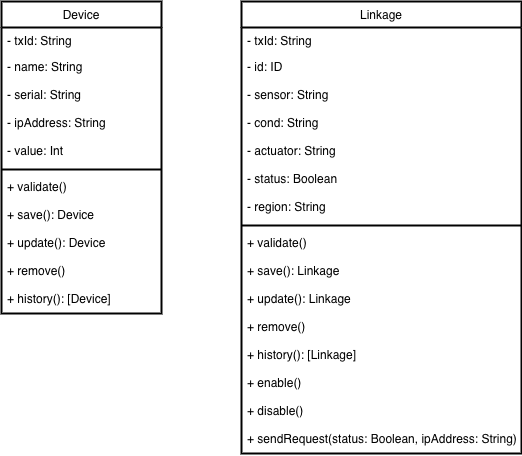
\includegraphics[width=10cm]{imagenes/diagramas/diagrama_clases}
    \caption{Diagrama de clases.}
    \label{fig:diagrama-de-clases}
\end{figure}

\subsubsection{Diagramas de secuencia.}

\begin{itemize}
    \item Listar dispositivos     
    
    \vspace{5mm}

    \begin{figure}[h!]
        \centering
        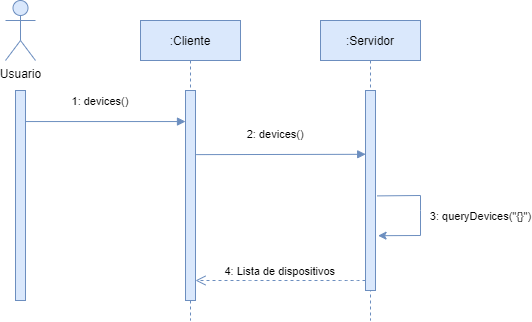
\includegraphics[width=10cm]{imagenes/diagramas/diagrama_secuencia_dispositivos}
        \caption{Diagrama de secuencia de Listar dispositivos.}
        \label{fig:secuencia-de-listar-dispositivos}
    \end{figure}

    \newpage

    \item Consultar dispositivo     
    
    \vspace{5mm}

    \begin{figure}[h!]
        \centering
        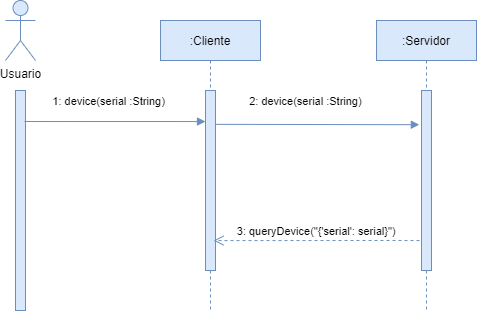
\includegraphics[width=10cm]{imagenes/diagramas/diagrama_secuencia_dispositivo}
        \caption{Diagrama de secuencia de Consultar dispositivo.}
        \label{fig:secuencia-de-consultar-dispositivo}
    \end{figure}

    \item Historial dispositivo     
    
    \vspace{5mm}

    \begin{figure}[h!]
        \centering
        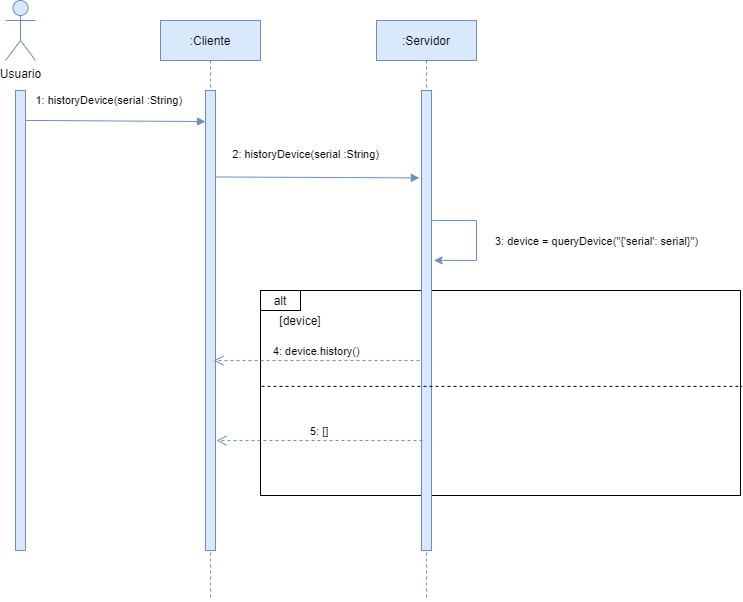
\includegraphics[width=10cm]{imagenes/diagramas/diagrama_secuencia_historiad}
        \caption{Diagrama de secuencia de Historial dispositivo.}
        \label{fig:secuencia-de-historial-dispositivo}
    \end{figure}

    \newpage

    \item Añadir dispositivo     
    
    \vspace{5mm}

    \begin{figure}[h!]
        \centering
        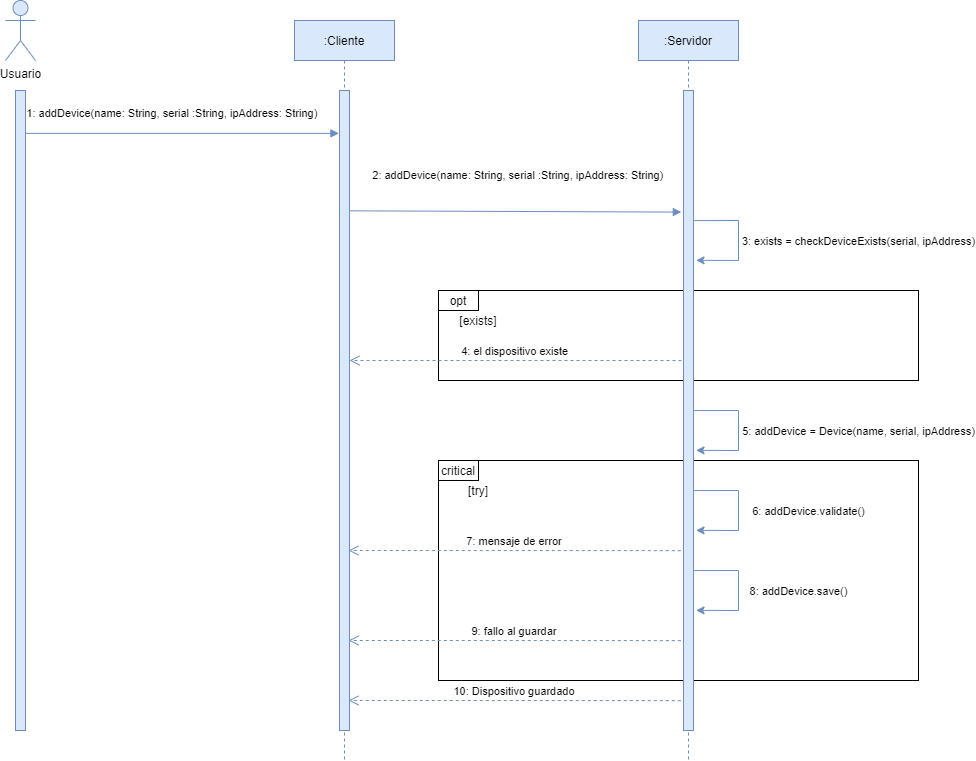
\includegraphics[width=10cm]{imagenes/diagramas/diagrama_secuencia_aniadird}
        \caption{Diagrama de secuencia de Añadir dispositivo.}
        \label{fig:secuencia-de-aniadir-dispositivo}
    \end{figure}

    \item Establecer valor a dispositivo     
    
    \vspace{5mm}

    \begin{figure}[h!]
        \centering
        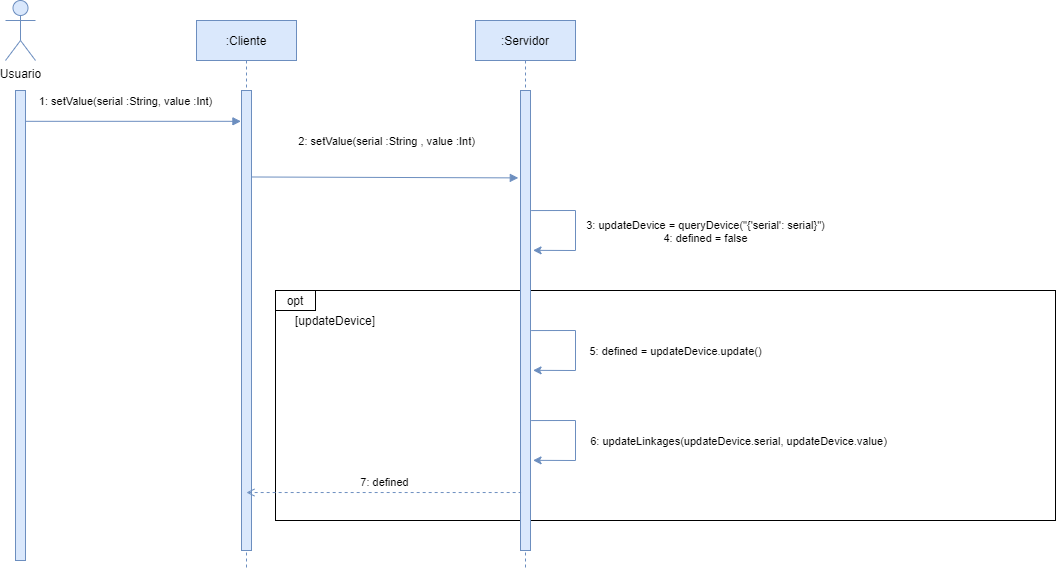
\includegraphics[width=10cm]{imagenes/diagramas/diagrama_secuencia_valor}
        \caption{Diagrama de secuencia de Establecer valor a dispositivo.}
        \label{fig:secuencia-de-establecer-valor-dispositivo}
    \end{figure}

    \newpage

    \item Borrar dispositivo     
    
    \vspace{5mm}

    \begin{figure}[h!]
        \centering
        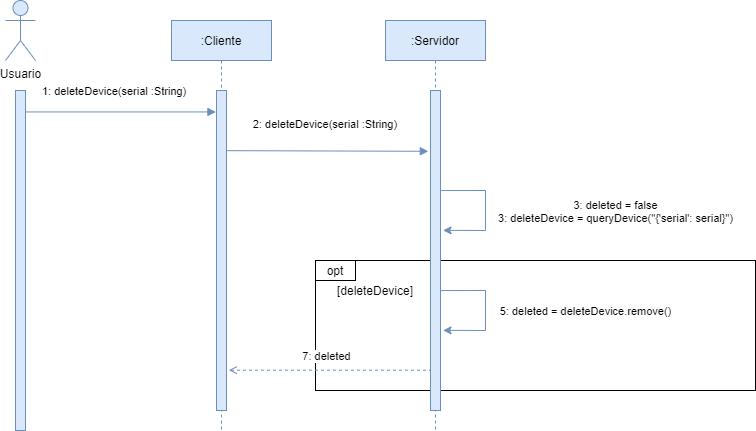
\includegraphics[width=10cm]{imagenes/diagramas/diagrama_secuencia_borrard}
        \caption{Diagrama de secuencia de Borrar dispositivo.}
        \label{fig:secuencia-de-borrar-dispositivo}
    \end{figure}

    \item Listar enlaces     
    
    \vspace{5mm}

    \begin{figure}[h!]
        \centering
        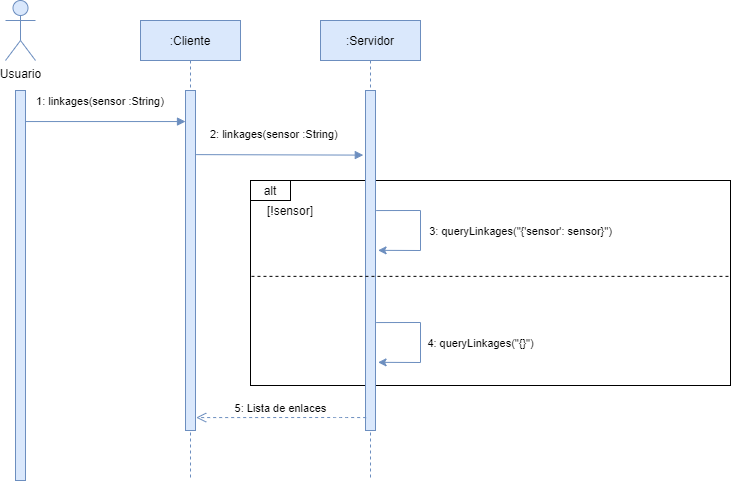
\includegraphics[width=10cm]{imagenes/diagramas/diagrama_secuencia_enlaces}
        \caption{Diagrama de secuencia de Listar enlaces.}
        \label{fig:secuencia-de-listar-enlaces}
    \end{figure}

    \newpage

    \item Consultar enlace     
    
    \vspace{5mm}

    \begin{figure}[h!]
        \centering
        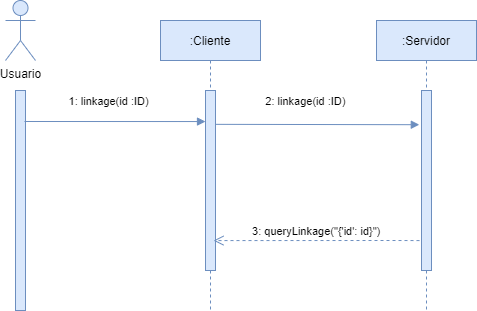
\includegraphics[width=10cm]{imagenes/diagramas/diagrama_secuencia_enlace}
        \caption{Diagrama de secuencia de Consultar enlace.}
        \label{fig:secuencia-de-consultar-enlace}
    \end{figure}

    \item Historial enlace     
    
    \vspace{5mm}

    \begin{figure}[h!]
        \centering
        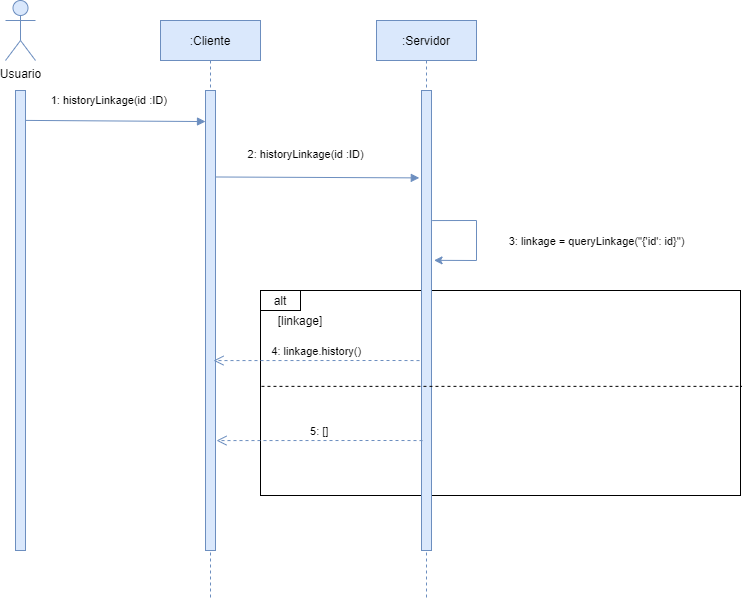
\includegraphics[width=10cm]{imagenes/diagramas/diagrama_secuencia_historiae}
        \caption{Diagrama de secuencia de Historial enlace.}
        \label{fig:secuencia-de-historial-enlace}
    \end{figure}

    \newpage

    \item Añadir enlace     
    
    \vspace{5mm}

    \begin{figure}[h!]
        \centering
        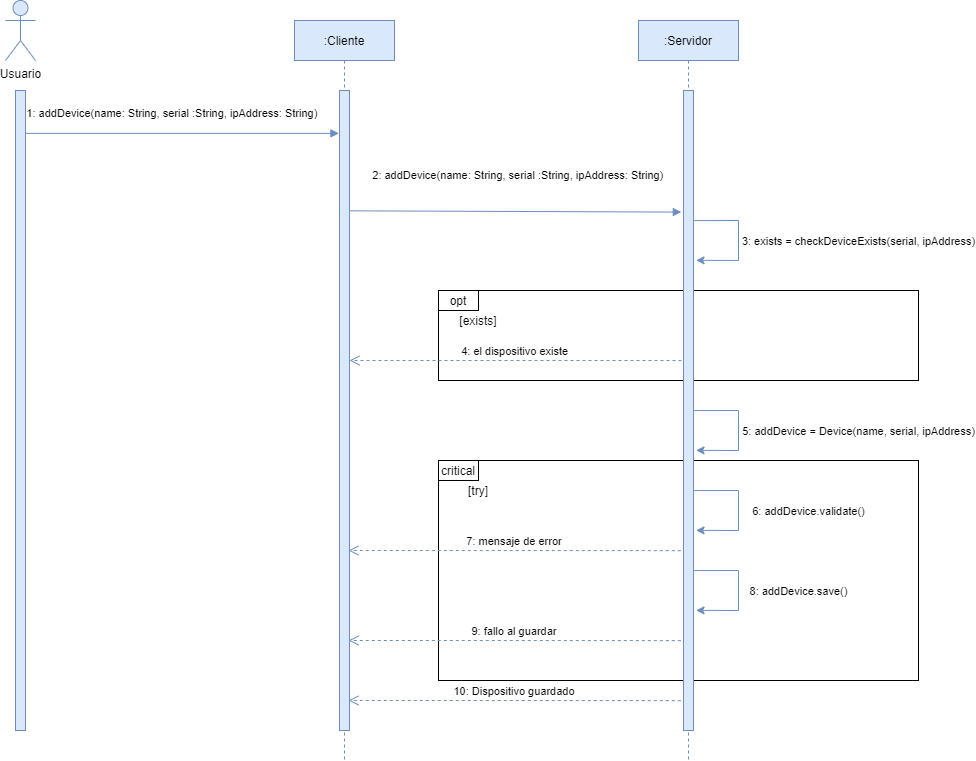
\includegraphics[width=10cm]{imagenes/diagramas/diagrama_secuencia_aniadird}
        \caption{Diagrama de secuencia de Añadir enlace.}
        \label{fig:secuencia-de-aniadir-enlace}
    \end{figure}

    \item Actualizar enlace     
    
    \vspace{5mm}

    \begin{figure}[h!]
        \centering
        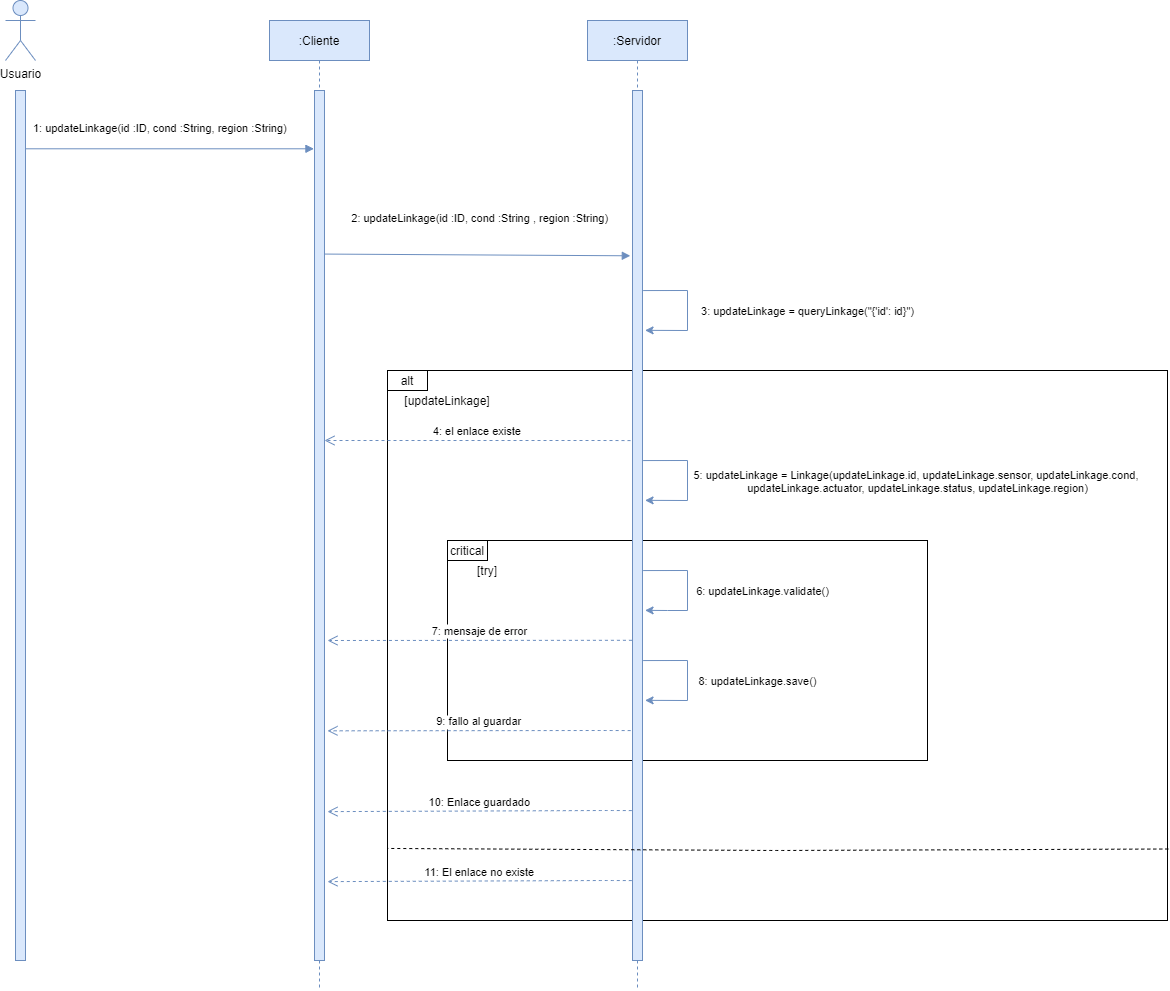
\includegraphics[width=10cm]{imagenes/diagramas/diagrama_secuencia_actualizar}
        \caption{Diagrama de secuencia de Actualizar enlace.}
        \label{fig:secuencia-de-actualizar-enlace}
    \end{figure}

    \newpage

    \item Borrar enlace     
    
    \vspace{5mm}

    \begin{figure}[h!]
        \centering
        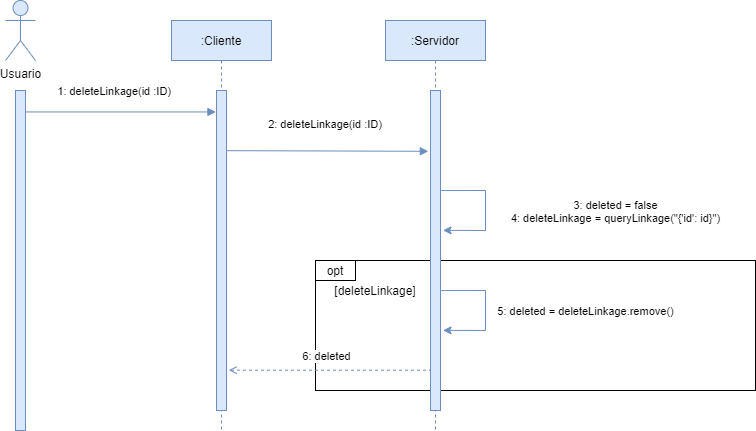
\includegraphics[width=10cm]{imagenes/diagramas/diagrama_secuencia_borrare}
        \caption{Diagrama de secuencia de Borrar enlace.}
        \label{fig:secuencia-de-borrar-enlace}
    \end{figure}

    \item Habilitar enlace     
    
    \vspace{5mm}

    \begin{figure}[h!]
        \centering
        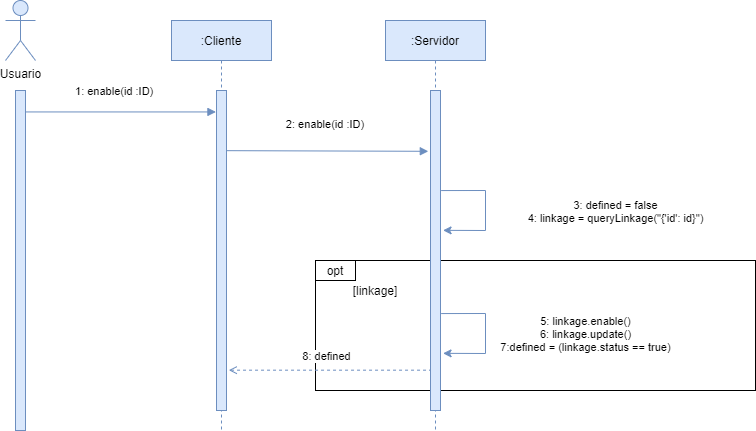
\includegraphics[width=10cm]{imagenes/diagramas/diagrama_secuencia_enable}
        \caption{Diagrama de secuencia de Habilitar enlace.}
        \label{fig:secuencia-de-habilitar-enlace}
    \end{figure}

    \newpage

    \item Deshabilitar enlace     
    
    \vspace{5mm}

    \begin{figure}[h!]
        \centering
        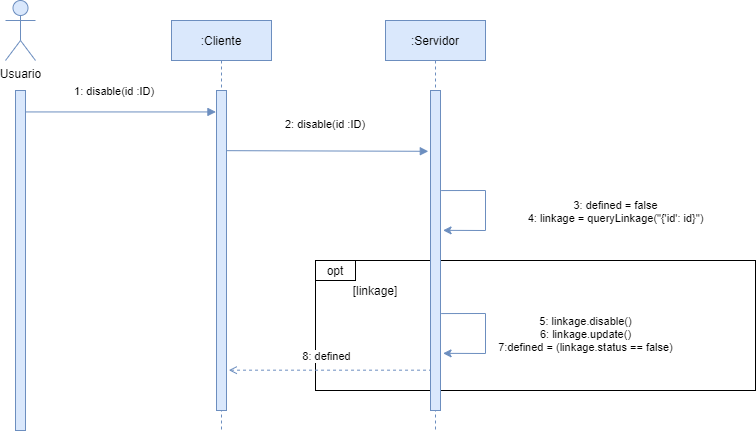
\includegraphics[width=10cm]{imagenes/diagramas/diagrama_secuencia_disable}
        \caption{Diagrama de secuencia de Deshabilitar enlace.}
        \label{fig:secuencia-de-deshabilitar-enlace}
    \end{figure}
\end{itemize}

\subsection{Planificación y presupuesto del proyecto.}

\subsubsection*{Planificación}

Después de explicar sobre el análisis de requerimientos, vamos a tratar sobre la planificación llevada a cabo en este 
proyecto y el presupuesto con el coste de desarrollo del mismo.

\vspace{5mm}

\noindent La planificación del proyecto se puede dividir en cuatro partes principalmente, que se puede reflejar en el 
siguiente diagrama de Gantt (ver fig. \ref{fig:planificacion-general}). La planificación consta de un proceso de 
investigación y lecturas de trabajos anteriores, libros, comparativa de plataformas Blockchain, etc. Por otro lado, se 
dedicó un plazo de tiempo en el aprovisionamiento de dispositivos hardware para la elaboración de la prueba de concepto y 
su posterior configuración e instalación del sistema operativo.

\vspace{5mm}

\noindent Antes de pasar a la implementación de la red, era necesario realizar una labor de investigación para la creación 
de los binarios e imágenes Docker de Hyperledger Fabric, para las arquitecturas ARM. Después de realizar modificaciones en 
el propio código de base de Hyperledger Fabric \cite{fork-fabric-baseimage}, implementé la red Blockchain en las Raspberry PI, 
que se puede encontrar en la rama \say{config-network} de mi repositorio \cite{repo}. A esta parte se dedicó cerca de más 
de 3 meses por la complejidad que tiene Hyperledger Fabric, ya que era muy difícil encontrar soluciones a determinados 
problemas que tenía durante la elaboración, además de la poca información acerca de la implementación de la red en máquinas 
como las utilizadas. Por lo tanto, tuve que dedicar un tiempo en implementar la red en mi máquina local y luego 
transladarlo a los nodos. Todo ello se puede ver en la rama \say{dev} del repositorio \cite{repo}. 

\vspace{5mm}

\noindent En la fase de análisis y diseño, se obtuvo los requisitos y los casos de uso del proyecto, para elaborar un 
boceto de la lógica de la aplicación. También se buscaron herramientas para elaborar las partes del Back end y el Front end, 
con sus principales ventajas y desventajas.

\vspace{5mm}

\noindent Para la fase de la implementación de la aplicación se dedicaron cerca de 2 meses y medio, para elaborar la API, 
creando los Resolvers, Schemas y Models para los enlaces y dispositivos, y su posterior conexión a la red Blockchain. Se 
creó un script para levantar el servicio en el nodo maestro y para poder hacerlo accesible desde fuera, se obtuvo un 
dominio mediante DDNS en la plataforma NO-IP \cite{no-ip}, y se abrieron los puertos 80 y 443 del router personal.

\vspace{5mm}

\noindent Para la implementación de la interfaz de usuario, se llevó a cabo la implementación de PWA, que usa HTTPS, tiene 
que incluir un manifiesto de Aplicación Web y debe de implementar un trabajador de servicio. Se desarrollaron las 
funcionalidades de enlaces y dispositivos, se conectó a la API y se realizaron test unitarios. Por último se desplegó en el 
servicio de Gatsby Cloud, que permite hacer análisis de SEO con la herramienta LightHouse.

\vspace{5mm}

\noindent Se puede obtener una planificación más detallada, extendiendo cada una de las partes elaboradas en la siguiente
página (ver fig. \ref{fig:planificacion-general}).

\begin{landscape}
  \begin{figure}[h!]
    \centering
    \vspace*{\fill}
    \noindent
    \makebox[0pt]{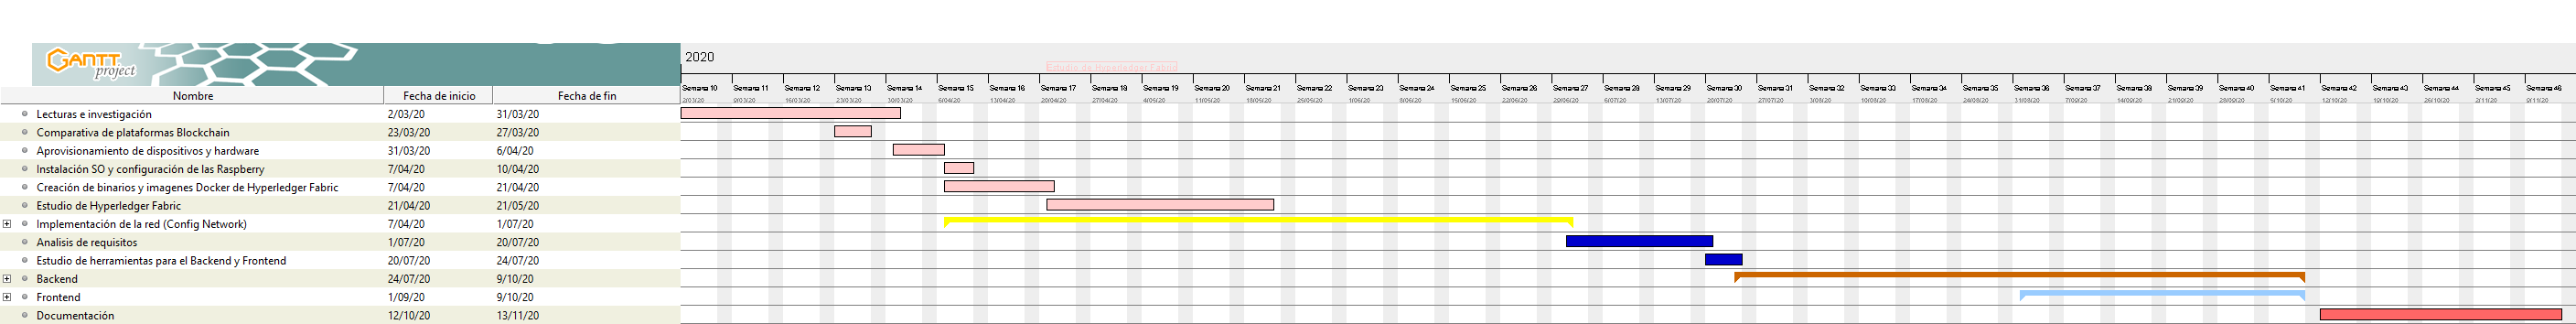
\includegraphics[width=1.2\paperwidth]{imagenes/planificacion/planificacion_general}}
    \caption{Planificación general.}
    \label{fig:planificacion-general}
    \vspace*{\fill}
  \end{figure}

  \begin{figure}[h!]
    \centering
    \vspace*{\fill}
    \noindent
    \makebox[0pt]{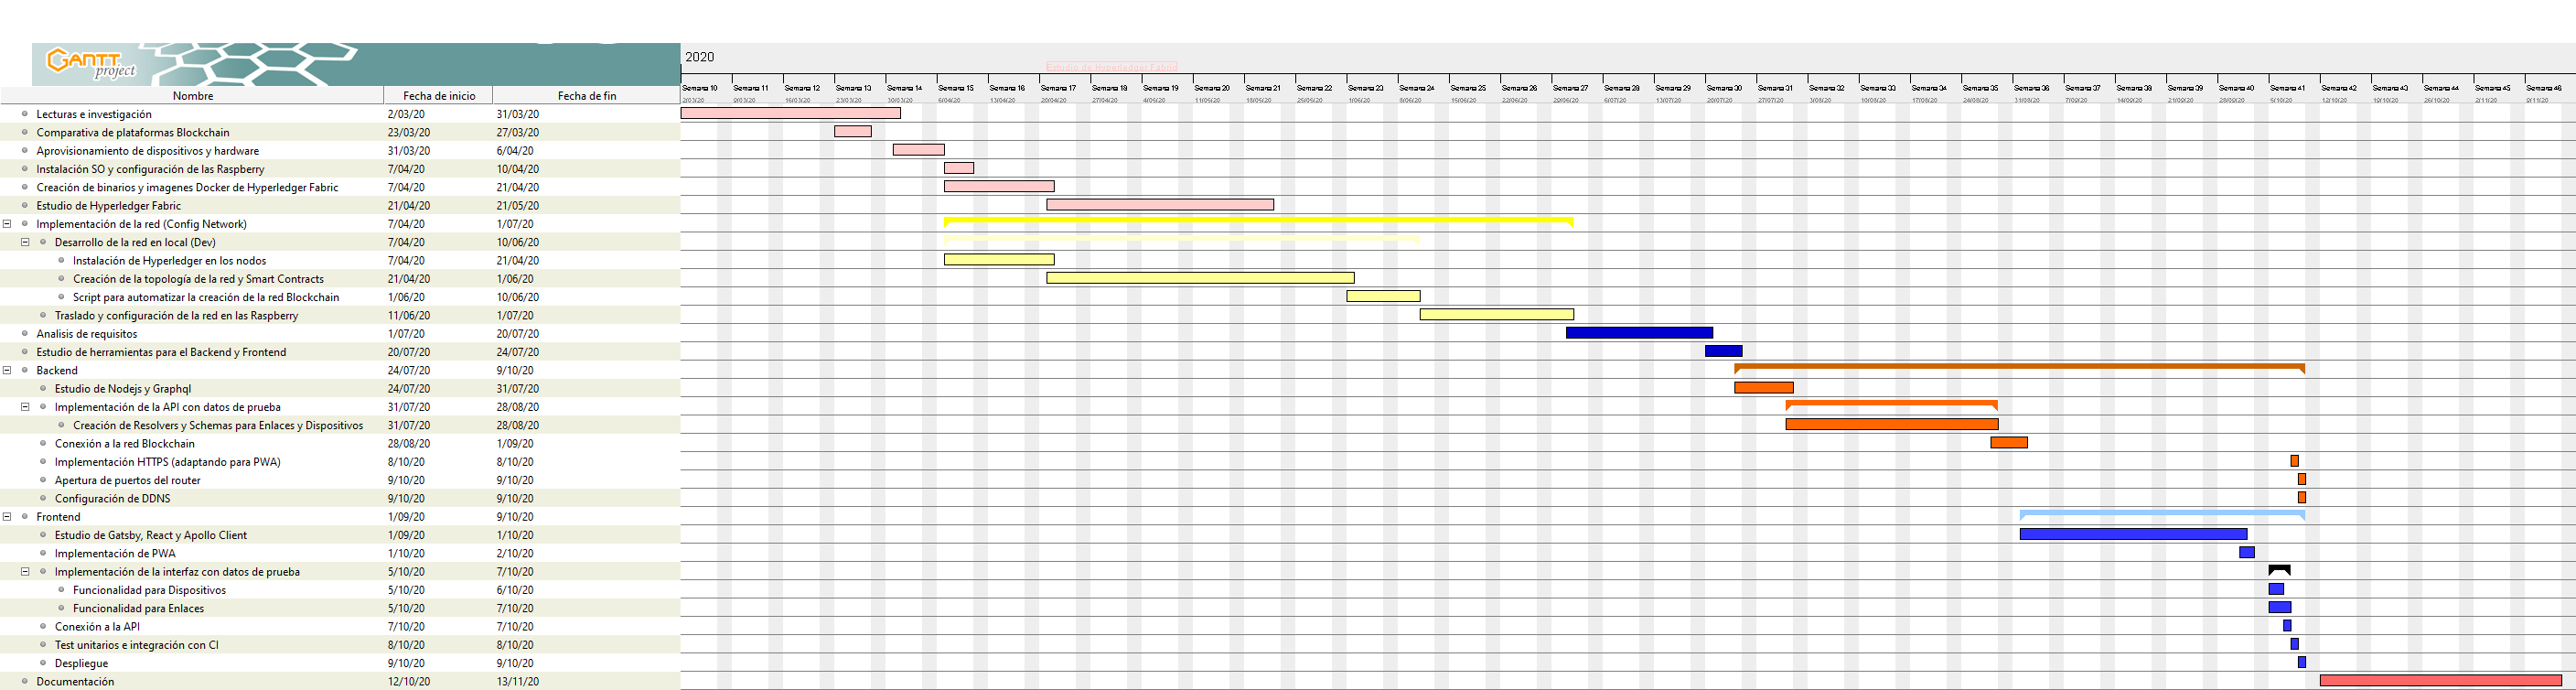
\includegraphics[width=1.2\paperwidth]{imagenes/planificacion/planificacion_expandida}}
    \caption{Planificación expandida.}
    \label{fig:planificacion-expandida}
    \vspace*{\fill}
  \end{figure}
\end{landscape}

\subsubsection*{Presupuesto}

Seguidamente, pasaremos hablar sobre el presupuesto para la realización del proyecto, teniendo en cuenta que se van a 
invertir 9 meses en él, desde el diseño de la plataforma hasta el despliegue y mantenimiento del mismo.

El calculo del presupuesto se va a valorar en función de los siguientes recursos:

\begin{itemize}
  \item Recurso humano.
  
  Se va a necesitar: 
  
  \begin{itemize}
    \item Jefe de proyecto, para que coordine las tareas del proyecto.
    \item Analista de sistemas, para que diseñe la plataforma, teniendo en cuenta los requerimientos del usuario.
    \item Full Stack Developer, para elaborar la implementación tanto del Back end y el Front end y su despliegue.
    \item Desarrollador Blockchain, encargado de la creación, gestión y mantenimiento de la red Blockchain.
  \end{itemize}

  Coste:

  \begin{table}[h!]
    \centering
    \begin{tabular}{|l|c|}
        \hline
        \textbf{Perfil}                     &   \textbf{Coste} \\
        \hline 
        \hline
        \textbf{Jefe de proyecto}           &   40.000 / 12 meses x 9 meses = 30.000€ \\ 
        \hline 
        \textbf{Analista de sistemas}       &   36.000 / 12 meses x 3 meses = 9.000€ \\ 
        \hline
        \textbf{Full Stack Developer}       &   30.000 / 12 meses x 6 meses = 15.000€ \\ 
        \hline
        \textbf{Desarrollador Blockchain}   &   40.000 / 12 meses x 4 meses = 13.333€ \\ 
        \hline
        \textbf{Coste total:}               &   30.000 + 9.000 + 15.000 + 13.333 = 67.333€ \\ 
        \hline
    \end{tabular}
    
    \caption{Coste de recursos humanos. Fuente: \cite{info-jobs}.}
    \label{table:coste-recurso-humanos}
  \end{table}


  \item Recurso material.

  Se ha utilizado: 
  
  \begin{itemize}
    \item Portatil: MacBook Pro 2018 con procesador 2,7 GHz Intel Core i7 de 4 núcleos de 
    16 GB de RAM y con capacidad de 256 GB. 1500€
    \item 5 Raspberry Pi: 
    5 Raspberries Pi (50€ cada una):
    \begin{itemize}
      \item 3 Raspberries Pi 4 Modelo B+ 2GB, que servirán como nodos principales para la red.
      \item Actuador (Raspberry Pi 2 Modelo B+) y sensor (Raspberry Pi 3 Modelo B+) para simular la red domótica.
    \end{itemize}
    \item Un switch TP-Link TL-SG105 - Switch 5 Puertos 10/100/1000 MBps 17,99€
    \item Cables ethernet: 14 €
    \item Xiaomi Router 4A WiFi inalámbrico 2.4GHz 5GHz Banda Dual 1167Mbps WiFi Repeater 4 Antenas 34,99 €
  \end{itemize}
  
  \item Otros gastos:
  \begin{itemize}
    \item Internet y Luz: 132 € x 9 meses = 1.188€
    \item Servicios de la nube: Utilizo la subscripción gratuita de Gatsby Cloud.
    \item Software: 0€
  \end{itemize}

  Coste total material: 3.004,98€
\end{itemize}

\begin{table}[h!]
  \centering
  \begin{tabular}{|l|c|}
      \hline
      \textbf{Recurso}  &   \textbf{Coste} \\
      \hline
      \hline 
      \textbf{Humano}   &   67.333€ \\ 
      \hline 
      \textbf{Material} &   3.004,98€\\ 
      \hline
      \textbf{Total}    &   70.337,98€\\ 
      \hline
  \end{tabular}
  
  \caption{Coste total de los recursos}
  \label{table:coste-recursos}
\end{table}

\newpage